\documentclass{article}
\usepackage[utf8]{inputenc}
\usepackage{amsmath}
\usepackage{geometry}
\geometry{
 a4paper,
 total={182mm,257mm},
 left=14mm,
 top=20mm,
 }
 \usepackage{amsthm}
 \usepackage[utf8]{inputenc}
 \usepackage[italian]{babel}
\usepackage[T1]{fontenc}
\usepackage{amssymb}
\usepackage{physics}
\usepackage{commath}
\usepackage{tikz}
\usepackage{pgfplots}
\usepackage{graphicx}
\graphicspath{ {Immagini/} }
\usepackage{float}
\usepackage{hyperref}
\hypersetup{
    colorlinks=true,
    linkcolor=red,
    citecolor=green
    filecolor=magenta,      
    urlcolor=cyan,
}


%Theorem Environments
\newtheorem{thm}{Teorema}[section]
\newtheorem{lem}[thm]{Lemma}
\newtheorem{property}{Proprietà}[section]
\newtheorem{defn}{Definizione}[section]
\newtheorem{prop}[defn]{Proposizione}
\newtheorem{example}{Esempi}[subsection]
\newtheorem{exerc}[example]{Esercizi Svolti}

%Commandi di Formattazione
\newcommand{\noi}{\noindent}
\newcommand{\note}{\noindent {\quad \bf \underline{Osservazione:}} \quad}
\newcommand{\eg}{\noindent {\bf \underline{Esempio:}} \quad}
\newcommand{\bfemph}[1]{\textbf{\textit{#1}}}
\renewcommand{\emph}[1]{\bfemph{#1}}

%Number Sets
\newcommand{\R}{\mathbb{R}}
\newcommand{\C}{\mathbb{C}}
\newcommand{\Z}{\mathbb{Z}}
\newcommand{\Q}{\mathbb{Q}}

%Shortcuts
\newcommand{\then}{\ensuremath{\Rightarrow}}
\newcommand{\twopartdef}[4]
{
	\left\{
		\begin{array}{ll}
			#1 & \mbox{se } #2 \\
			#3 & \mbox{se } #4
		\end{array}
	\right.
}

%Vectors
\renewcommand{\i}{\vu{i}}
\renewcommand{\j}{\vu{j}}
\renewcommand{\k}{\vu{k}}
\renewcommand{\a}{\va{a}}
\renewcommand{\b}{\va{b}}
\renewcommand{\c}{\va{c}}
\renewcommand{\v}{\va{v}}
\renewcommand{\u}{\va{u}}
\newcommand{\s}{\va{s}}
\renewcommand{\t}{\va{t}}
\newcommand{\verst}{\vu{t}}
\newcommand{\versr}{\vu{r}}
\renewcommand{\r}{\va{r}}
\newcommand{\tauvs}{\vu{\tau}}
\newcommand{\tauvt}{\va{\tau}}
\newcommand{\normvs}{\vu{n}}
\newcommand{\N}{\va{N}}
\newcommand{\g}{\va{g}}
\newcommand{\F}{\va{F}}
\newcommand{\f}{\va{f}}
\newcommand{\M}{\va{M}}
\renewcommand{\l}{\va{l}}
\newcommand{\p}{\va{p}}
\renewcommand{\P}{\va{P}}
\renewcommand{\L}{\va{L}}


\renewcommand{\c}{\overline{c}}
\title{Appunti Lezioni}
\author{Roberto Gargiulo}
\date{Ultimo Aggiornamento: \today}


\begin{document}

\maketitle
\tableofcontents
\pagebreak

\section{Lezioni di Meccanica II Semestre}

\subsection{Forze d'Attrito - 5 Marzo (L)}

Ricapitolazione delle \textbf{Reazioni Vincolari}:
\begin{center}
\begin{tabular}{c|c|c|c}
    Forza & Intensità & Direzione & Verso \\
    \hline
    Tensione $\va{\tau}$ & ? & Lungo il Filo & Interno al Filo\\
    Normale $\va{N}$ & ? & Perpendicolare alla Superficie di Contatto & Opposto alla compenetrazione\\
    Forza d'Attrito Radente $\va{f_a}$ & ? & Lungo la Superficie di Contatto & Dipende dalle condizioni di equilibrio\\
    \hline
\end{tabular}
\end{center}

Notiamo che fintanto che la situazione di equilibrio è statica allora la forza d'attrito equilibra perfettamente la forza risultante parallela alla superficie di contatto tra due corpi. Graficamente ciò si traduce in una retta di inclinazione $\frac{\pi}{4}$, sperimentalmente si dimostra che per ogni materiale esiste un certo coefficiente $\mu_S$ tale che se $|\F_\parallel|=|\f_a|>\mu_S|\N|$ (dove $\N$ è la normale) allora la situazione passa da un \textbf{regime statico} ad uno \textbf{dinamico} in cui la forza d'attrito ha valore costante minore di $\mu_S|\N|$ e uguale a $\mu_d|\N|$ dove $\mu_d$ è il \textbf{coefficiente d'attrito dinamico}.

\begin{example}
\begin{enumerate}
    \item Equilibrio delle Forze su un corpo appoggiato su un piano orizzontale liscio.
    \item Risultante delle Forze su un corpo appoggiato su un piano inclinato liscio.
    \item Risultante delle Forze su un corpo appoggiato su un piano inclinato con attrito.
\end{enumerate}
\end{example}

Dall'ultimo esempio possiamo ricavare la condizione affinchè su un piano inclinato con attrito un corpo in stato di quiete rimanga in tale stato:
\[\i) -|\f_a|+mg\sin\alpha=0\]
\[\j) |\N|-mg\cos\alpha=0\]
Allora otteniamo:
\[|\f_a|\leq \mu_S|\N|\iff mg\sin\alpha\leq \mu_Smg\cos\alpha\iff \boxed{\tan\alpha\leq \mu_S}\]

Consideriamo il caso dinamico ($\tan\alpha>\mu_S$):
\begin{enumerate}
    \item Il corpo si trova ad un carta quota h e viene spinto dalla forza-peso lungo il piano inclinato. Scelto un riferimento tale che ha origine nella posizione iniziale del corpo uno degli assi parallelo al piano inclinato e diretto verso il basso, l'altro perpendicolare e uscente dal piano, otteniamo:
    \[-\mu_dmg\cos\alpha+mg\sin\alpha=ma\iff a=g(\sin\alpha-\mu_d\cos\alpha) \]
    Poniamo poi \(\sin\alpha-\mu_d\cos\alpha=\lambda^-\)
    \item Il corpo viene spinto con una certa velocità $\v_0$ parallela al piano inclinato (scelto il riferimento che ha origine nella posizione iniziale del corpo, un asse parallelo al piano e diretta verso l'alto, l'altro perpendicolare uscente):
    \[-\mu_dmg\cos\alpha-mg\sin\alpha=ma\iff a=-g(\sin\alpha+\mu_d\cos\alpha) \]
    Poniamo poi \(\sin\alpha\mu_d\cos\alpha=\lambda^+\)
\end{enumerate}
Consideriamo il primo caso. Scriviamo le leggi orarie (posto $t_0=0$) e consideriamo la velocità dopo una certa quota h:
\[a(t)=g\lambda^-\then v(t)=g\lambda^-t\then x(t)=\frac{g\lambda^-}{2}t^2\]
Quindi raggiunta una certa quota h allora x(t) sarà:
\[x(t)=\frac{h}{\sin\alpha}=\frac{g\lambda^-}{2}t^2\iff \overline{t}=\sqrt{\frac{2h}{g\lambda^-\sin\alpha}}\then \boxed{v(\overline{t})=\sqrt{\frac{2hg\lambda^-}{\sin\alpha}}}\]

\begin{exerc}[Unità B]
\begin{enumerate}
    \item \(\left[1.12\right]\) - Corpo lanciato con velocità iniziale (verso l'alto) lungo un piano inclinato con attrito (noti i coefficienti d'attrito): scelto un sistema di riferimento appropriato, determinare le leggi orarie della I fase (fino a fermarsi) e della II fase (durante la caduta); (nota la velocità iniziale)determinare l'angolo di inclinazione del piano affinchè il corpo torni nella posizione originale con velocità dimezzata; trovato tale angolo, si pone $\alpha'=\frac{\alpha}{2}$ e si dimostri che il corpo si ferma e quale distanza percorre.
    \item \(\left[1.13\right]\) - Corpi collegati attraverso un filo e una carrucola poggiati su un doppio piano inclinato (note le masse, i coefficienti d'attrito di entrambi i lati del piano e le inclinazioni): determinare l'accelerazione con la quale si muovono i corpi e la tensione del filo.
\end{enumerate}
\end{exerc}


\subsection{Forza Elastica e Oscillatore Armonico - 7 Marzo (L)}

Data una molla ai cui estremi sono attaccati dei corpi si osserva \underline{sperimentalmente} che esiste un regime detto \textbf{regime di Hooke} in cui è valida la \textbf{legge di Hooke} che stabilisce:
\begin{align}
\label{leggehooke}
    |\f_e|=k|l-l_0|=k|\Delta l|\\
    \f_e\parallel \i
\end{align}
Dove k è la costante elastica, $l_0$ la lunghezza della molla a riposo ed $l$ la lunghezza della molla dopo la deformazione.
Il verso invece è tale da opporsi alla deformazione della molla. In particolare fissato un estremo, ad esempio quello sinistro, mentre quello destro è lasciato libero di muoversi, si ottiene:
\begin{enumerate}
    \item Nel riferimento centrato nel riferimento fisso e orientato verso destra allora:
    \[\f)-k(x(t)-l_0)\i\]
    \item Nel riferimento centrato nella posizione del corpo in stato di riposo della molla:
    \[\f=-kx(t)\i\]
\end{enumerate}
Indipendentemente dal sistema di riferimento è sempre valido però:
\[\Delta l=x_B-x_A-l_0\]

Studiamo quindi il moto di un corpo collegato all'estremo destro di una molla poggiato su un piano liscio, fissando il sistema di riferimento nella posizione di riposo del corpo. Otteniamo quindi la seguente equazione di forze:
\[\N+\f_e+m\g=m\a\]
Allora proiettando sull'asse delle ascisse:
\[(f_e)_x=ma\]
Allora per quanto detto otteniamo:
\[-kx=m\ddot{x}\]
Ossia un'equazione differenziale lineare di secondo ordine omogenea a coefficienti costanti:
\[\ddot{x}+\frac{k}{m}x=0\]
Per ricondurci alla soluzione già nota del moto armonico operiamo la seguente sostituzione:
\[\Omega=\sqrt{\frac{k}{m}}\then \ddot{x}+\Omega^2x=0\]
Allora due soluzione linearmente indipendenti sono $\sin(\Omega t),\cos(\Omega t)$ e quindi una generica soluzione al problema può ossere ottenuta come combinazione lineare:
\[x(t)=c_1\sin(\Omega t)+c_2\cos(\Omega t)\]
Fissate le condizioni iniziali $x(0)=x_0,v(0)=v_0$ possiamo calcolare $c_1,c_2$:
\begin{align*}
    x(0)=c_2=x_0\\
    \Dot{x}(0)=c_1\Omega=v_0\then c_1=\frac{v_0}{\Omega}
\end{align*}
Ottenendo quindi la funzione:
\begin{equation}
    \boxed{x(t)=\frac{v_0}{\Omega}\sin(\Omega t)+x_0\cos(\Omega t)}
\end{equation}
Tale funzione si può esprimere anche sotto la forma:
\begin{equation}
    x(t)=A\sin(\Omega t+\phi)=A\sin(\Omega t)\cos\phi+A\cos(\Omega t)\sin\phi
\end{equation}
Fissando:
\[c_1=A\cos\phi\quad c_2=A\sin\phi\]
Mentre rispetto alle condizioni iniziali otteniamo le seguenti formule:
\[A=\sqrt{x_0^2+\frac{v_0^2}{\Omega^2}}\quad \tan\phi=\frac{x_0\Omega}{v_0}\]
Possiamo quindi esplicitare le leggi orarie di posizione e velocità nella prima forma, più immediata per considerare casi particolari di condizioni iniziali:
\[\left\{\begin{array}{l}
    x(t)=\frac{v_0}{\Omega}\sin(\Omega t)+x_0\cos(\Omega t) \\
    \Dot{x}(t)=v_0\cos(\Omega t)-x_0\Omega\sin(\Omega t)  \\
\end{array}\right.\iff
\left\{\begin{array}{l}
    x(t)=A\sin(\Omega t+\phi) \\
    \Dot{x}(t)=A\Omega\cos(\Omega t +\phi)  \\
\end{array}\right.\]

\paragraph{Casi Particolari}

Nel caso $x(0)=x_0\neq0,v(0)=0$ otteniamo:
\[A=\sqrt{x_0^2}=x_0\quad \phi=\frac{\pi}{2}\]
E quindi le equazioni diventano:
\[\left\{\begin{array}{l}
    x(t)=x_0\cos(\Omega t) \\
    \Dot{x}(t)=-x_0\Omega\sin(\Omega t)  \\
\end{array}\right.\]

Nel caso $x(0)=0,v(0)=v_0\neq0$ otteniamo:
\[A=\frac{v_0}{\Omega}\quad\phi=0\]
E quindi:
\[\left\{\begin{array}{l}
    x(t)=\frac{v_0}{\Omega}\sin(\Omega t) \\
    \Dot{x}(t)=v_0\cos(\Omega t)\\
\end{array}\right.\]

\subsubsection{Oscillatore Armonico "Non Omogeneo}
Consideriamo il caso di una molla appesa verticalmente al soffitto a cui è attaccato un corpo, allora la risultante delle forze è:
\[\F=m\g+\F_e\]
Siccome agiscono tutte lungo l'asse verticale, fissando l'origine nella posizione a riposo della molla e orientandolo verso il basso otteniamo le seguenti proiezioni:
\[mg-kz=m\ddot{z}\]
Ossia la seguente equazione differenziale:
\[\ddot{z}+\frac{k}{m}z=g\]
Quindi ponendo $\Omega=\sqrt{\frac{k}{m}}$ otteniamo un'equazione differenziale lineare a coefficienti costanti di second'ordine ma non omogenea:
\[\ddot{z}+\Omega z=g\]
Che ha per soluzioni una combinazione lineare dell'omogenea associata più una soluzione particolare, che è in tal caso $\frac{g}{\Omega^2}$:
\[x(t)=c_1\sin(\Omega t)+c_2\cos(\Omega t)+\frac{g}{\Omega^2}=A\sin(\Omega t+\phi)+\frac{g}{\Omega^2}\]
Usando la prima forma e imponendo le condizioni iniziali $x(0)=x_0,v(0)=v_0$ otteniamo:
\[\left\{\begin{array}{l}
    x(t)=\frac{v_0}{\Omega}\sin(\Omega t)+\left(x_0-\frac{g}{\Omega^2}\right)\cos(\Omega t)+\frac{g}{\Omega^2} \\
    \Dot{x}(t)=v_0\cos(\Omega t)-\left(x_0-\frac{g}{\Omega^2}\right)\Omega\sin(\Omega t)  \\
\end{array}\right.\]
Mentre possiamo passare alla seconda forma usando le seguenti formule:
\[A=\sqrt{\left(x_0-\frac{g}{\Omega^2}\right)^2+\left(\frac{v_0}{\Omega}\right)^2}\quad\tan\phi=\Omega\frac{x_0-\frac{g}{\Omega^2}}{v_0}\]

\paragraph{Casi Particolari}
Consideriamo il caso in cui $x(0)=x_0\neq0,v(0)=0$ otteniamo quindi:
\[A=x_0-\frac{g}{\Omega^2}\quad \phi=\frac{\pi}{2}\]
E quindi le equazioni diventano:
\[\left\{\begin{array}{l}
    x(t)=\left(x_0-\frac{g}{\Omega^2}\right)\cos(\Omega t)+\frac{g}{\Omega^2} \\
    \Dot{x}(t)=-\left(x_0-\frac{g}{\Omega^2}\right)\Omega\sin(\Omega t)  \\
\end{array}\right.\]

Nel caso in cui $x(0)=0,v(0)=v_0\neq0$ otteniamo:
\[A=\frac{v_0}{\Omega}\quad\phi=\arctan\left(-\frac{g}{v_0\Omega}\right)\]
E quindi le leggi oraria:
\[\left\{\begin{array}{l}
    x(t)=\frac{v_0}{\Omega}\sin(\Omega t)-\frac{g}{\Omega^2}\cos(\Omega t)+\frac{g}{\Omega^2} \\
    \Dot{x}(t)=v_0\cos(\Omega t)+\frac{g}{\Omega}\sin(\Omega t)  \\
\end{array}\right.\]
Mentre nel caso $x(0)=0,v(0)=0$ otteniamo:
\[\left\{\begin{array}{l}
    x(t)=\frac{g}{\Omega^2}\left(1-\cos(\Omega t)\right) \\
    \Dot{x}(t)=\frac{g}{\Omega}\sin(\Omega t)  \\
    \ddot{x}(t)=g\cos(\Omega t)
\end{array}\right.\]
Tale funzione ha il seguente grafico:
\begin{figure}[H]
    \centering
    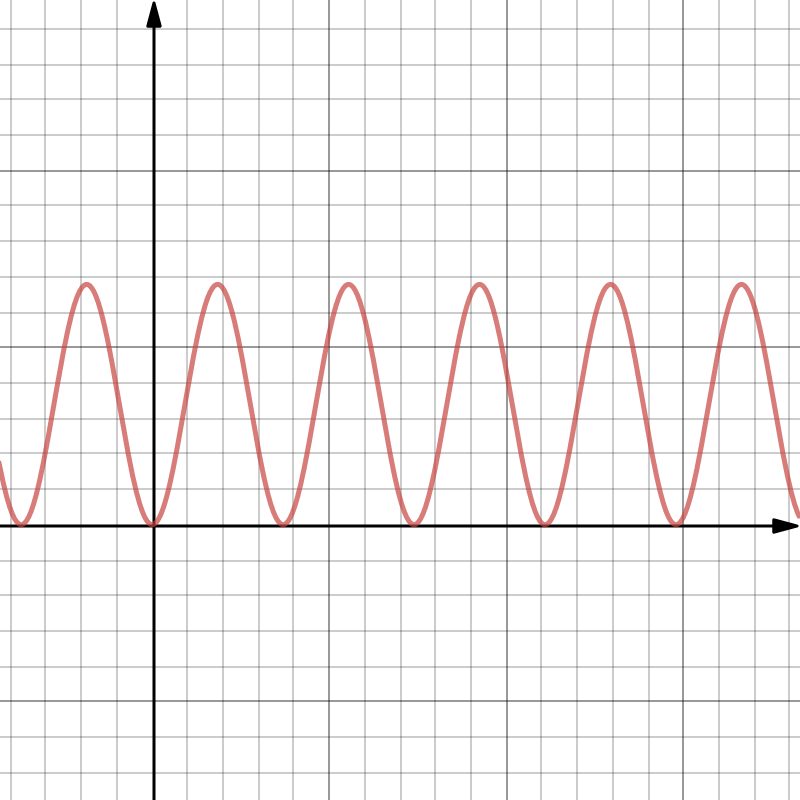
\includegraphics[width=0.5\textwidth]{Immagini/Appunti/desmos-graph.png}
    \label{grafomollaconpeso}
\end{figure}
Esso va interpretato come segue: dalla posizione di riposo il corpo cade fino a raggiungere il punto in cui la forza elastica e la forza peso coincidono, quindi l'accelerazione è nulla; a questo punto la forza elastica è maggiore della forza peso e rallenta il corpo fino a farlo fermare, il corpo allora risale finchè la forza elastica e la forza peso non si eguagliano, mentre il corpo continua ad avanzare con la velocità che aveva accomulato in risalita mentre viene rallentato fino a fermarsi e così via.



\subsubsection{Corpo Appoggiato ad una Molla Compressa su Piano Scabro}
Consideriamo quindi la risultante delle forze:
\[m\ddot{x}=\mu_dmg-kx\]
A cui riconduciamo la seguente equazione differenziale ponendo $\Omega=\sqrt{\frac{k}{m}}$:
\[\ddot{x}+\Omega^2x=-\mu_dg\]
La I Fase (ossia fino alla posizione di riposo) è la stessa che si è presentata nel caso precedente sostituendo $g$ con $-\mu_dg$:
\[\left\{\begin{array}{l}
    x(t)=\frac{v_0}{\Omega}\sin(\Omega t)+\left(x_0+\frac{\mu_dg}{\Omega^2}\right)\cos(\Omega t)-\frac{\mu_dg}{\Omega^2} \\
    \Dot{x}(t)=v_0\cos(\Omega t)-\left(x_0+\frac{\mu_dg}{\Omega^2}\right)\Omega\sin(\Omega t)  \\
\end{array}\right.\]
La II Fase del moto è invece un moto uniformemente decelerato con velocità e iniziale:
\[m\ddot{x}=-\mu_dmg\then \ddot{x}=-\mu_dg\]
\[\left\{\begin{array}{l}
    x(t)=v_0(t-t_0)-\frac{\mu_dg}{2}(t-t_0)^2  \\
    \Dot{x}(t)=v_0-\frac{\mu_d}{g}(t-t_0)  \\
\end{array}\right.\]
Notiamo inoltre che siccome la fase di distacco avviene quando la molla raggiunge la posizione di riposo allora la posizione iniziale della II fase sarà sicuramente $x(0)=0$.\\
\note Utilizzando la seconda forma possiamo inoltre stabilire una relazione "senza tempo" direttamente tra velocità e posizione:
\begin{equation}
    A^2=\left(x+\frac{\mu_d}{g}\right)^2+\frac{v^2}{\Omega^2}\then \boxed{v=\Omega\sqrt{A^2-\left(x_0+\frac{\mu_dg}{\Omega^2}\right)^2}}
\end{equation}

\subsection{I Moti Relativi - 9 Marzo (S)}
Consideriamo due sistemi di riferimento K e K', il primo dei quali per comodità definiamo "fisso" o anche "assoluto" in quanto tutte le nostre osservazioni partiranno da tale riferimento. Allora nell'osservare il moto di un corpo che nel sistema K ha posizione $\r(t)$ e posizione $\r'(t)$ in K' allora si verifica la seguente equazione:
\[\r(t)=\r'(t)+\r_{O'}(t)\]
Dove $\r{O'}(t)$ è la posizione istante per istante del centro di riferimento di K' rispetto a K. Graficamente:
\begin{figure}[H]
    \centering
    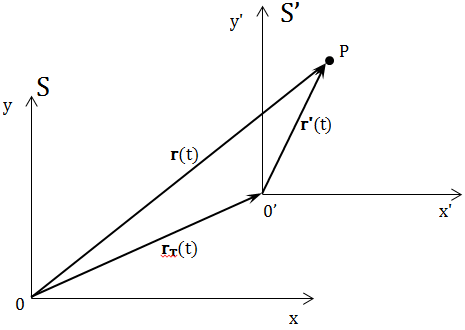
\includegraphics{Appunti/image20.png}
    \caption{Il Sistema "Fisso" (Assoluto) e quello "Mobile" (Relativo)}
    \label{motirelativi}
\end{figure}
Mentre per rispetto alle velocità otteniamo:
\[\dv{\r}{t}=\dv{\r'}{t}+\dv{r_{O'}}{t}\iff \v(t)=\v'(t)+\v_T(t)\]
Dove $\v_T$ è detta \textbf{velocità di trascinamento} e si può calcolare esplicitando in componenti:
\[\r(t)=\r'(t)+\r_{O'}(t)\iff x(t)\i+y(t)\j+z(t)\k=x'(t)\i'(t)+y'(t)\j'(t)+z'(t)\k'(t)+x_{O'}(t)\i+y_{O'}(t)\j+z_{O'}(t)\k\]
Ricordando che si può definire un certo vettore $\va{\omega}$ di "rotazione" tale che:
\[\dv{\i}{t}=\omega\times\i\]
E inoltre tutti i versori ruotano secondo lo stesso "vettore":
\[\i'\cdot\k'=0\then \dv{(\i'\cdot\k')}{t}=0\then \dv{\i'}{t}\cdot\k'+\i'\cdot\dv{\k'}{t}=0\then (\va{\omega}\times\i')\cdot\k'+\i'\cdot(\va{\omega'}\times\k')=(\i'\times\k')\cdot\va{\omega}+\va{\omega'}(\k'\times\i')=\]\[(\i'\times\k')\cdot\va{\omega}-\va{\omega'}(\i'\times\k')=\va{\omega}\cdot(\k'\times\i')-\va{\omega'}(\i'\times\k')=(\va{\omega}-\va{\omega'})(\i'\times\k')=(\va{\omega}-\va{\omega'})\j'=0\iff \va{\omega}=\va{\omega'}\]
Possiamo quindi derivare:
\begin{equation}
\begin{split}
    \dot{x}(t)\i+\dot{y}(t)\j+\dot{z}(t)\k&=\dv{\left[x'(t)\i'(t)+y'(t)\j'(t)+z'(t)\k'(t)\right]}{t}+\dv{\left[x_{O'}(t)\i+y_{O'}(t)\j+z_{O'}(t)\k\right]}{t}=\\
    &=\dot{x'}(t)\i'+\dot{y'}(t)\j'+\dot{z'}(t)\k'+x'(t)\dot{\i}'+y'(t)\dot{\j}'+z'(t)\dot{\k}'+\dot{x}_{O'}(t)\i+\dot{y}_{O'}(t)\j+\dot{z}_{O'}(t)\k=\\
    &=\dot{x'}(t)\i'+\dot{y'}(t)\j'+\dot{z'}(t)\k'+x'(t)(\va{\omega}\times\i')+y'(t)(\va{\omega}\times\j')+z'(t)(\va{\omega}\times\k')+\dot{x}_{O'}(t)\i+\dot{y}_{O'}(t)\j+\dot{z}_{O'}(t)\k=\\
    &=\v'(t)+\va{\omega}(t)\times\r'(t)+\v_{O'}(t)=\boxed{\v'(t)+\v_T(t)}
\end{split}
\end{equation}
Applichiamo lo stesso ragionamento per le accelerazioni e otteniamo:
\begin{equation}
\begin{split}
    \a(t)&=\dv{\v'(t)}{t}+\dv{\v_{O'}(t)}{t}+\dv{(\va{\omega}\times\r'}{t}=\\  &=\a'(t)+\va{\omega}\times\v'+\a_{O'}(t)+\dv{\va{\omega}}{t}\times\r'+\va{\omega}\times\dv{\r'}{t}=\\
    &=\a'(t)+\va{\omega}\times\v'+\a_{O'}(t)+\dv{\va{\omega}}{t}\times\r'+\va{\omega}\times(\v'(t)+\va{\omega}\times\r')=\\
    &=\a'(t)+\va{\omega}\times\v'+\a_{O'}(t)+\dv{\va{\omega}}{t}\times\r'+\va{\omega}\times\v'(t)+\va{\omega}\times\va{\omega}\times\r'=\\
    &=\a'(t)+\a_{O'}(t)+\dot{\va{\omega}}\times\r'+\va{\omega}\times\va{\omega}\times\r'+2\va{\omega}\times\v'=\boxed{\a'(t)+\a_T(t)+\a_{C}(t)}\\
\end{split}
\end{equation}
Dove $\a_T(t)$ è l'accelerazione di Trascinamento e $\a_{Co}=2\va{\omega}\times\v'$ è l'accelerazione di Coriolis. 

\paragraph{I Sistemi Inerziali}
\begin{defn}
Un \textbf{Sistema Inerziale} è un Sistema in cui i valgono le Leggi di Newton (i tre principi della dinamica), ossia tale che la risultante di tutte le forze agenti sul sistema è nulla.
\end{defn}
Data come ipotesi che esiste un tale riferimento K, consideriamo un altro sistema K' che si muove di moto traslatorio uniforme rispetto a K, osservando che:
\[a_{O'}(t)=0\quad\va{\omega}=0\then \a(t)=\a'(t)\]
E in particolare se $\a=0\then \a'=0$ e quindi la risultante delle forze agenti su K' è nulla se è nulla in K, quindi anche K' è un sistema inerziale. Abbiamo quindi dimostrato che un qualunque sistema che si muove di moto rettilineo uniforme rispetto ad un sistema inerziale è anch'esso inerziale.
Possiamo però fare un passo ulteriore, in quanto avendo derivato le formule di composizione delle accelerazioni possiamo calcolare il valore della "forza apparente":
\[\a=\a'+\a_T+\a_C\then m\a=m\a'+m(\a_T+\a_C)\then \F=\F'+\f\]
Dove $\F$ è la risultante delle forze reali agenti sul corpo, $\F'$ è la risultante delle forze misurate dal sistema K' agenti sul corpo ed $\f$ è il "termine correttivo" o anche "\textbf{forza apparente}" in quanto non è esercitata da alcuna sorgente/interazione. Essa vale:
\[\f=\F'-\F=\boxed{-m\left[\a_{O'}(t)+\dot{\va{\omega}}\times\r'+\va{\omega}\times\va{\omega}\times\r'+2\va{\omega}\times\v'\right]}\]
Ossia in un sistema inerziale non osserveremo necessariamente la validità di $\F=m\a$ e quindi se $\F=0$ non è detto che $\a=0$ e quindi che il corpo si muova di moto rettilineo uniforme, da cui \textit{non} inerziale.


\subsection{Pendolo Semplice con Attrito - 12 Marzo (L)}
Studiamo il moto di un pendolo che si muove con piccole oscillazioni ed è soggetto ad un'attrito viscoso del tipo $\F=-b\v$ allora la risultante delle forze:
\[\tauvt+m\g-b\v=m\a\]
E proiettando lungo gli assi equiversi ai versori normale $\normvs$ e tangente $\tauvs$:
\begin{equation}
\left\{
\begin{array}{l}
    mg\cos\theta-\tau=-ml\Dot{\theta}^2  \\
    -mg\sin\theta-bl\Dot{\theta}=ml\ddot{\theta}  \\ 
\end{array}\right.
\end{equation}
Che si riduce per piccole oscillazioni a:
\begin{equation}
\left\{
\begin{array}{l}
    mg\cos\theta-\tau=-ml\Dot{theta}^2  \\
    -mg\theta-bl\Dot{\theta}=ml\ddot{\theta}  \\ 
\end{array}\right.
\end{equation}
Quindi otteniamo un'equazione differenziale in $\theta(t)$ lineare di second'ordine a coefficienti costanti omogenea:
\[\ddot{\theta}+\frac{b}{m}\Dot{\theta}+\frac{g}{l}\theta=0\]
La quali si può risolvere ricorrendo all'equazione caratteristica associata:
\[\lambda^2+\frac{b}{m}\lambda+\frac{g}{l}=0\]
Risolvendo otteniamo le seguenti soluzioni:
\[\lambda_{1,2}=-\frac{b}{2m}\pm\sqrt{\frac{b^2}{4m^2}-\frac{g}{l}}\]
Da cui possiamo ricavare tre tipologie di soluzioni a seconda del segno del discriminante:
\[\begin{array}{l}
     \Delta>0\then x(t)=c_1e^{\lambda_1t}+c_2e^{\lambda_2t}  \\
      \Delta=0\then x(t)=c_1e^{\lambda_0}+c_2te^{\lambda_0t}\\
      \Delta<0\then x(t)=c_1e^{\alpha t}\cos(\beta t)+c_2e^{\alpha t}\sin(\beta t)
\end{array}\]
Dove $\alpha,\beta$ sono rispettivamente la parte reale e la parte immaginaria (entrambe prese in valore assoluto) delle due soluzioni (complesse coniugate).
Analizziamo uno per uno i casi.\\
\paragraph{Smorzamento Sovracritico}
Per $\Delta>0$ l'attrito viscoso è tanto alto da annullare quasi completamente il moto:
\begin{figure}[H]
    \centering
    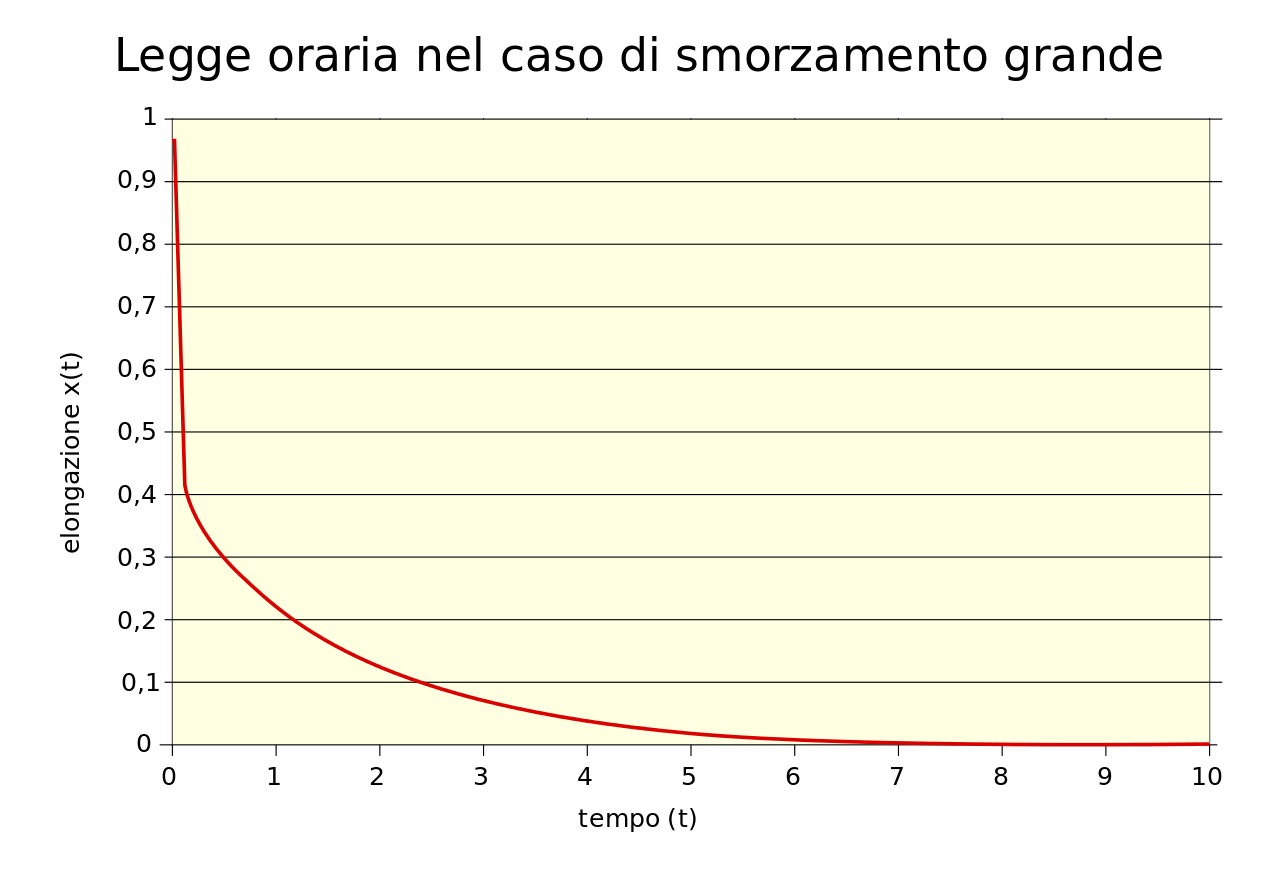
\includegraphics[width=0.5\textwidth]{Appunti/SmorzamentoSovracritico.png}
    \label{sovrasmorz}
\end{figure}
\pagebreak
\paragraph{Smorzamento Critico}
Quando $\Delta=0$ otteniamo un simile risultato, con una piccola oscillazione iniziale seguita da uno smorzamento che annulla il moto all'infinito:
\begin{figure}[H]
    \centering
    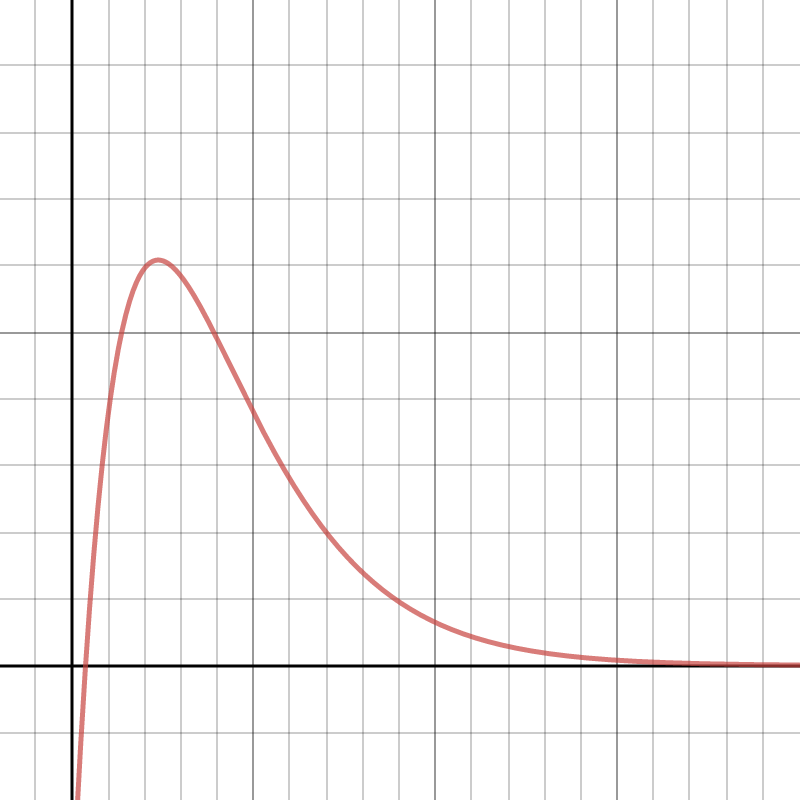
\includegraphics[width=0.5\textwidth]{Appunti/SmorzamentoCritico.png}
    \label{smorzcritico}
\end{figure}
\paragraph{Sottosmorzamento}
Quando $\Delta<0$ allora l'attrito non è tale da ridurre drasticamente il comportamento "oscillatorio" del corpo, ma comunque all'infinito le oscillazioni si annullano:
\begin{figure}
    \centering
    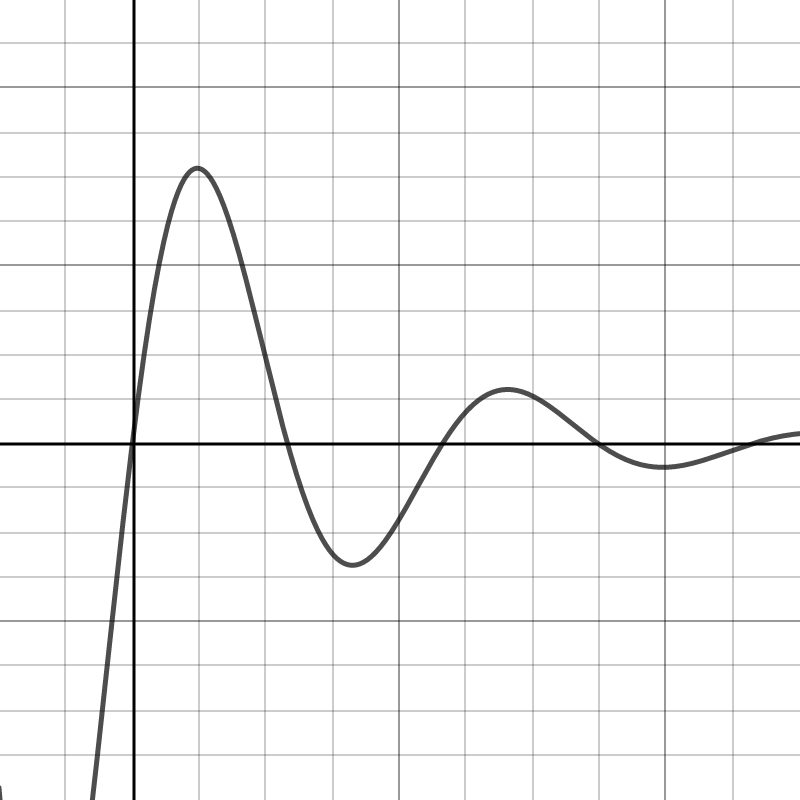
\includegraphics[width=0.5\textwidth]{Appunti/SottoSmorzamento.png}
    \label{sottosmorz}
\end{figure}


\subsection{Potenza, Lavoro ed Energia - 21 Marzo (S)}
\begin{defn}
La \textbf{potenza} sviluppata da una forza $\F$ si definisce come il prodotto scalare tra la forza $\F(t)$ e la velocità $\v(t)$:
\[W(t)=\F(t)\cdot\v(t)\]
\end{defn}

\begin{thm}[Il Teorema delle Forze Vive]
Data una forza $\F$ applicata ad un corpo che si muove di velocità $\v(t)$, la potenza sviluppata dalla forza vale:
\begin{equation}
\begin{split}
    W(t)=\F(t)\cdot\v(t)&=m\dv{\v(t)}{t}\v(t)=\\
    &=m\frac{1}{2}\dv{\v(t)\cdot\v(t)}{t}=\frac{1}{2}m\dv{|\v(t)|^2}{t}=\\
    &=\boxed{\dv{t}\left(\frac{1}{2}mv^2\right)}
\end{split}    
\end{equation}
Definiamo la quantità $\frac{1}{2}mv^2$ \textbf{energia cinetica} K di un corpo di massa m che si muove con velocità di modulo v.
\end{thm}
\begin{defn}
Il \textbf{lavoro} compiuto dalla forza $\F$ in un intervallo $\Delta t=t_2-t_1$ si definisce come:
\begin{equation}
    \mathbb{L}(t_1,t_2)=\int_{t_1}^{t_2}W(t)\dd t=\int_{t_1}^{t_2}\F(t)\cdot\v(t)\dd t
\end{equation}
\end{defn}
\begin{thm}[Il Teorema del Lavoro e dell'Energia Cinetica]
Per il teorema della forze vive possiamo esplicitare la potenza sviluppata da $\F$ come derivata dell'energia cinetica rispetto al tempo:
\begin{equation}
    \mathbb{L}(t_1,t_2)=\int_{t_1}^{t_2}W(t)\dd t=\int_{t_1}^{t_2}\dv{K(t)}{t}\dd t=\int_{t_1}^{t_2}\dd K=K(t_2)-K(t_1)=K_2-K_1=\Delta K
\end{equation}
Ossia il lavoro compiuto da una forza implica una variazione di energia.
\end{thm}
\paragraph{Formulazione Alternativa del Lavoro}
Notiamo che esplicitando il lavoro secondo la sua definizione e a sua volta esplicitando la velocità come derivata del raggio vettore siamo in grado di ricondurre la definizione di lavoro come integrale di Riemann della potenza rispetta al tempo ad un integrale di linea della forza rispetto alla traiettoria:
\[\mathbb{L}(t_1,t_2)=\int_{t_1}^{t_2}W(t)\dd t=\int_{t_1}^{t_2}\F(t)\cdot\v(t)\dd t=\int_{t_1}^{t_2}\F(t)\cdot\dv{\r}{t}\dd t=\int_{P_1}^{P_2}\F(\r)\dd\r\]
Ponendo $P_1=\r(t_1),P_2=\r(t_2)$ e riscrivendo $\F$ in funzione di $\r$ invece che di t.
Possiamo inoltre ricondurre nuovamente questo integrale ad uno di Riemann ricordando la definizione di prodotto scalare in $V_3$:
\[\mathbb{L}(t_1,t_2)=\int_{P_1}^{P_2}\F\cdot\dd\r=\int_{P_1}^{P_2}|\F|\cos\alpha(s)|\dd \r|=\int_{P_1}^{P_2}|\F(s)|\cos\alpha(s)\dd s\]
Dove $s(t)$ è l'ascissa curvilinea, che si può invertire ($t=t(s)$)in modo da poter scrivere anche $\F$ in funzione di $s(t)$.
Le differenze principali tra queste formulazioni sono i diversi usi, la prima è più comoda da trattare analiticamente ed è utile quando è nota la velocità/posizione istante per istante mentre la seconda - sebbene più complicata - è particolarmente utile quando tutto ciò che è noto è la traiettoria e la forza in funzione di essa. Un esempio tipico è quello del lavoro fatto dalla tensione di un pendolo (non necessariamente semplice), in quanto siccome per le proprietà della circonferenza lo spostamento è perpendicolare alla tensione (radiale) in ogni punto allora ogni lavoro infinitesimo è nullo:
\[\dd\mathbb{L}=\tauvt\cdot\dd\r=0\then \mathbb{L}=\int\dd\mathbb{L}=0\]
\paragraph{Il Lavoro di più Forze}
Data la risultante delle forze $\F$:
\[\F=\F_1+\F_2+\F_3\]
Possiamo ottenere il lavoro esercitato dalla forza F come somma dei lavori esercitati da ciascuna forza:
\[\mathbb{L}=\int_{P_1}^{P_2}\F\dd\r=\int_{P_1}^{P_2}\left(\F_1+\F_2+\F_3\right)\dd\r=\int_{P_1}^{P_2}\F_1\dd\r+\int_{P_1}^{P_2}\F_2\dd\r+\int_{P_1}^{P_2}\F_3\dd\r=\mathbb{L_1}+\mathbb{L_2}+\mathbb{L_3}\]

\paragraph{Campi di Forza}
\begin{defn}
Un \textbf{Campo di Forze} è una funzione $\F(\r)$ che associa ad ogni punto di una certa zona dello spazio un vettore $\F(\r)$.
\end{defn}
\begin{example}
Un esempio tipico è il campo gravitazionale che, nelle nostre approssimazioni, è uniforme (nello spazio) e costante (nel tempo).
\end{example}
Nei campi di forze ha senso quindi parlare di \textbf{lavori virtuali}, ossia il lavoro compiuto dalla forza $\F$ su una certa traiettoria $\gamma'$ contenuta nella parte di spazio su cui è definito il campo vettoriale. In generale il lavoro virtuale di una traiettoria immaginaria è ben distinto dal lavoro effettivo, ma esistono particolari campi di forze in cui non è cosi.
\begin{defn}
Un \textbf{Campo di Forze Conservativo} è un campo tale che dati due punti $P_1,P_2$ allora il lavoro compiuto dalle forze su una qualunque traiettoria che collega tali punti è lo stesso:
\[\int_\gamma\F(\r)\dd\r=\int_{\gamma'}\F(\r)\dd\r\]
\end{defn}
Questa proprietà permette quindi di non dover conoscere la traiettoria scelta dal corpo, in quanto note le posizioni di partenza e d'arrivo è possibile scegliere una qualunque traiettoria (quindi la più comoda per i calcoli) ottenendo lo stesso risultato. Osserviamo inoltre che per le proprietà degli integrali e dei campi conservativi il lavoro svolto su una curva chiusa è sempre nullo:
\[ {}_{\gamma_1} \int_{P_1}^{P_2}\F(\r)\dd\r={}_{\gamma_2} \int_{P_1}^{P_2}\F(\r)\dd\r=-{}_{\gamma_2} \int_{P_2}^{P_1}\F(\r)\dd\r\then {}_{\gamma_1}\int_{P_1}^{P_2}\F(\r)\dd\r+{}_{\gamma_2} \int_{P_2}^{P_1}\F(\r)\dd\r=0 \]
Ciò equivale alla scrittura seguente, che esprime un integrale di linea lungo una curva chiusa:
\begin{equation}
    \boxed{{}_\gamma\oint\F(\r)\dd\r=0}
\end{equation}
Grazie a queste proprietà è possibile definire il lavoro come funzione dei soli punti $P_1,P_2$, a sua volta esprimibile come differenza di una certa funzione $U$ nel punto $P_1$ e nel punto $P_2$:
\[\mathbb{L}=\int_{P_1}^{P_2}\F(\r)\dd\r=V(P_1,P_2)=U(P_1)-U(P_2)=-\Delta U\]
Possiamo quindi definire la \textbf{variazione di energia potenziale} come l'opposto del lavoro necessario a spostare un corpo da una posizione $P_1$ ad una posizione $P_2$. Inoltre, similmente al lavoro, la variazione di energia totale è data dalla somma delle variazioni di energia totali:
\[\Delta U=-\mathbb{L}=-(L_1+L_2+L_3)=-L_1-L_2-L_3=\Delta U_1+\Delta U_2+\Delta U_3\]

\subsection{Campi di Forze Conservativi, Energia Meccanica - 26 Marzo (S)}
Consideriamo il lavoro compiuto dalla risultante delle forze su un certo corpo, notiamo che siccome possiamo scrivere:
\[\F=\F^C+\F^{NC}\]
Ossia la risultante delle forze è data dalla risultante delle forze conservative e non conservative. Possiamo scrivere quindi:
\[\mathbb{L}=\mathbb{L}^C+\mathbb{L}^{NC}\]
Per definizione di energia potenziale e per il teorema dell'energia cinetica otteniamo quindi:
\[\Delta K=-\Delta U+\mathbb{L}^{NC}\]
Che si può riscrivere come:
\[\Delta K+\Delta U=\Delta(K+U)=\mathbb{L}^{NC}\]
Definiamo quindi la somma di energia cinetica e potenziale l'\textbf{energia meccanica} di un corpo ottenendo l'enunciato del \textbf{Teorema Generale delle'Energia Meccanica}:
\begin{thm}
\begin{equation}
    \boxed{\Delta E=\mathbb{L}^{NC}}
\end{equation}
\end{thm}
Che nel caso in cui un corpo è soggetto solo a forze conservative oppure le forze non conservative sono a lavoro nullo (ossia del tipo $\F\perp\dd\r$) otteniamo la \textbf{Conservazione dell'Energia Meccanica}:
\begin{equation}
    \Delta E=0\iff E_1=E_2
\end{equation}
Notiamo inoltre che per la definizione di energia potenziale, la funzione $U(\r)$ è determinata a meno di una costante $c$ la quale è fissata scelto lo zero dell'energia potenziale (solitamente quando la forza responsabile del campo si annulla). 
Consideriamo quindi il lavoro infinitesimo, detto \textbf{forma differenziale}:
\[\dd L=\F(\r)\dd\r=F_x\dd x+F_y\dd y+F_x\dd z\]
Mentre la variazione infinitesima di energia potenziale si può dimostrare valere:
\[\dd U=\pdv{U}{x}\dd x+\pdv{U}{y}\dd y+\pdv{U}{z}\dd z\]
Per un campo conservativo si verifica quindi:
\[\dd \mathbb{L}=-\dd U\]
In termini vettoriali otteniamo:
\[\left(\pdv{U}{x},\pdv{U}{y},\pdv{U}{z}\right)=\grad{U}\]
Dove $\grad{U}$ è detto \textbf{Gradiente} del campo scalare U. E nel caso di un campo conservativo otteniamo che:
\[\F=\left(F_x,F_y,F_z\right)=-\left(\pdv{U}{x},\pdv{U}{y},\pdv{U}{z}\right)=-\grad{U}\then\boxed{ \F=-\grad{U}}\]

\paragraph{Energia Potenziale Elastica}
Consideriamo una molla che ha lunghezza a riposo $l_0$, fissando il sistema di riferimento nell'estremo fisso della molla, allora essa esercita una forza che proiettata sull'asse parallelo ad essa:
\[F_x=-k(x-l_0)\]
Calcoliamo quindi il lavoro esercitato dalla forza elastica su un corpo attaccato all'estremo libero della molla:
\[\mathbb{L}=-k\int_{x_1}^{x_2}F(x)\dd x=-k\eval{\left(x-l_0\right)^2}_{x_1}^{x_2}\]
Otteniamo quindi che in un percorso chiuso il lavoro totale è nullo, ossia il campo è conservativo:
\[\mathbb{L}=\oint F(x)\dd x=-k\eval{\left(x-l_0\right)^2}_{x_1}^{x_2}-k\eval{\left(x-l_0\right)^2}_{x_2}^{x_1}=0\]
Possiamo quindi definire a meno di una costante l'energia potenziale elastica:
\[U(x)=\frac{k}{2}(x-l_0)^2+c\]
Dove $c=0$ ponendo $U(l_0)=0$.

\paragraph{Equilibri Stabili e Instabili}
Consideriamo una forza conservativa (unidimensionale) la cui energia potenziale ha il seguente grafico:
\begin{figure}[H]
    \centering
    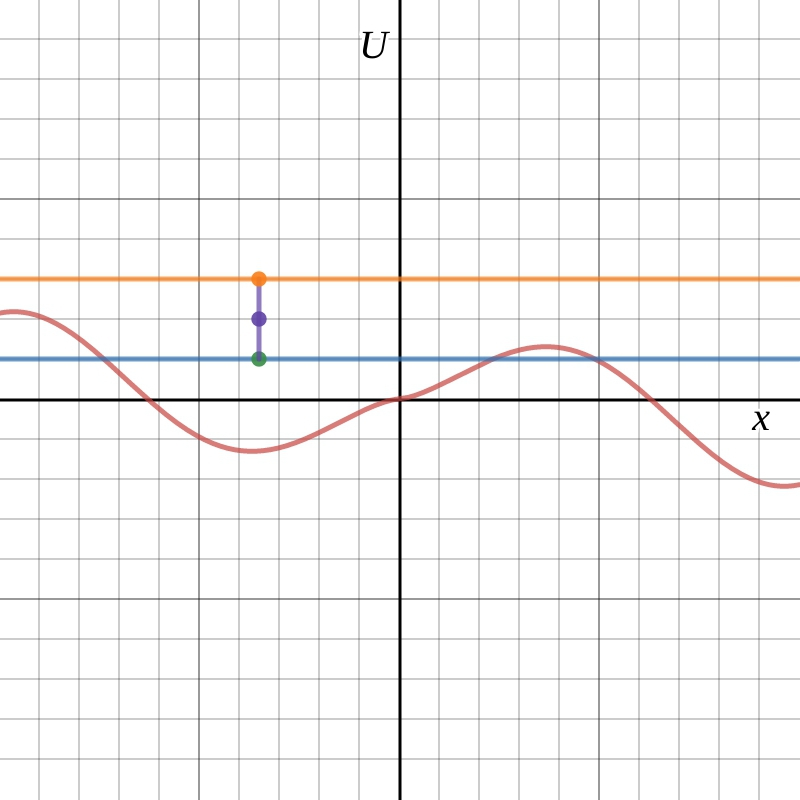
\includegraphics[width=0.4\textwidth]{Equilibri.jpg}
    \caption{Esempio di funzione U(x)}
    \label{equilibrienergiapotenziale}
\end{figure}

Nel caso in cui il corpo ha un energia meccanica $E_1$ (quella più bassa) il corpo tende a oscillare intorno al punto di minimo, mentre nel caso $E_2$ (quella più alta) il corpo è altamente instabile e "precipita" cercando il punto di minimo più vicino, per poi oscillarci intorno. Possiamo osservare ciò matematicamente considerando che ogni funzione derivabile due volte in un punto può essere approssimata da una parabola grazie al \textbf{polinomio di Taylor} all'interno della quale il corpo tende a oscillare.

Ritornando alla molla, calcoliamo energia potenziale e cinetica in funzione del tempo nota la soluzione all'equazione differenziale:
\[m\ddot{x}=-k(x-x_0)\then \ddot{y}+\omega y=0\quad\quad \omega=\sqrt{\frac{k}{m}}, y=x-l_0\]
E quindi otteniamo $y=A\sin(\omega t+\phi)$ e sostituendo nelle formule delle energie:
\begin{align*}
    K=\frac{1}{2}m\dot{y}^2=\frac{1}{2}m\omega^2 A^2\cos^2(\omega t+\phi)=\frac{1}{2}kA^2\cos^2(\omega t+\phi)\\
    U=\frac{1}{2}my^2=\frac{1}{2}mA^2\sin^2(\omega t+\phi)
\end{align*}
Quindi l'energia meccanica:
\[E=K+U=\frac{1}{2}kA^2\left(\sin^2(\omega t+\phi)+\cos^2(\omega t+\phi)\right)=\boxed{\frac{1}{2}kA^2}=cost\]
Che ci permette di collegare direttamente l'ampiezza del moto all'energia meccanica del corpo.

\paragraph{Energia Potenziale Gravitazionale}
Noto che $\F_P=m\g=m(0,0,-g)$ allora il lavoro esercitato dalla forza-peso è dato dalla sola componente verticale:
\[\mathbb{L}=-mg\int_{z_1}^{z_2}\dd z=-mg(z_2-z_1)\]
Definiamo quindi l'energia potenziale gravitazionale:
\[U(z)=mgz+c\]
\paragraph{Moto di un Proiettile}
Applichiamo quanto appena dimostrato per la forza-peso al moto di un proiettile, soggetto solo a tale forza:
\[E=\frac{1}{2}mv^2+mgz=\frac{1}{2}m(v_x^2+v_y^2)+mgz\]
Allora note le condizioni iniziali vogliamo calcolare la massima altezza, considerando che l'energia meccanica vale rispettivamete:
\begin{align*}
    E=\frac{1}{2}mv_0^2\\
    E=\frac{1}{2}mv_0^2\cos^2\theta+mgh_M
\end{align*}
Siccoma la forza-peso è conservativa:
\[\frac{1}{2}mv_0^2=\frac{1}{2}mv_0^2\cos\theta+mgh_M\then h_m=\frac{v_0^2-v_0^2\cos^2\theta}{2g}=\frac{v_0^2\sin\theta}{2g}\]
\paragraph{Pendolo}
Similmente al moto del proiettile, l'unica forza a lavoro non nullo agente su un pendolo è la forza peso (in quanto $\tauvt\perp\dd\r$), quindi otteniamo (ponendo il riferimento sul soffitto):
\[E=\frac{1}{2}mv^2+mgz=\frac{1}{2}ml^2\dot{\theta}^2+mgl(1-\cos\theta)\]
Quando raggiunge la posizione massima a $\theta_0$ otteniamo:
\[E=mgl(1-\cos\theta_0)\]
Quindi comparando entrambe le scritture siamo in grado di stabilire un espressione della velocità in funzione dell'angolo/posizione stesso invece che del tempo:
\[\frac{1}{2}ml^2\dot{\theta}^2+mgl(1-\cos\theta)=mgl(1-\cos\theta_0)\then\frac{1}{2}ml^2\dot{\theta}^2=mgl(\cos\theta-\cos\theta_0)\then \dot{\theta}=\sqrt{2\frac{g}{l}(\cos\theta-\cos\theta_0)} \]
Da cui risulta che necessariamente $\cos\theta\leq\cos\theta_0\iff \theta\leq\theta_0$
in $[0,\pi]$.
Possiamo inoltre approssimare per piccole oscillazioni l'energia meccanica del pendolo grazie al polinomio di Taylor:
\[\cos\theta=1-\frac{\theta^2}{2}+o(\theta^4)\then 1-\cos\theta=\frac{\theta^2}{2}+o(\theta^4)\]
Ottenendo:
\[E(\theta)=K(\dot{\theta})+U(\theta)=\frac{1}{2}ml^2\dot{\theta}^2+mgl(1-\cos\theta)\approx\frac{1}{2}ml^2\dot{\theta}^2+mgl\frac{\theta^2}{2}=\boxed{\frac{1}{2}ml[l\dot{\theta}^2+g\theta^2]}\]

\subsection{Campi Centrali e Momento Angolare - 6 Aprile (S)}

Si definisce \textbf{Campo Centrale} un Campo di Forze per cui, dato un centro O, la direzione della forza applicata in un qualunque punto dello spazio è sempre la congiungente tra quel punto e il centro O, tali forze possono essere sia repulsive che attrattive e si possono scrivere con la seguente formulazione:
\begin{equation}
    \boxed{\F(\r)=f(|\r|)\r}
\end{equation}
Un esempio tipico è la forza gravitazionale:
\[\F_g(\r)=G\frac{mM}{|\r|^3}\r\then f(|\r|)=G\frac{mM}{|\r|^3}\]
Il \textbf{momento di un vettore} rispetto ad un punto O si definisce come segue:
\begin{equation}
    \boxed{\M=\r\times\a}
\end{equation}
Dove $\r$ è il vettore posizione del punto in cui è applicato il vettore $\a$ rispetto ad O.
\begin{defn}[Momento Angolare]
Il momento angolare è il momento della quantità di moto:
\[\l_O=\r\times\p=\r\times(m\v)\]
\end{defn}
\begin{defn}[Momento di una Forza]
\[\M_O=\r\times\F\]
\end{defn}
\begin{property}[Variazione del Momento Angolare]
\begin{equation}
    \dv{\l_O}{t}=m\dv{\r\times\v}{t}=m\dv{\r}{t}\times\v+m\r\times\dv{\v}{t}=m(\v\times\v+\r\times\a)=\r\times(m\a)=\r\times\F=\M_O
\end{equation}
Ossia la variazione del momento angolare è determinata dall'azione di una forza esterna sul sistema.
\end{property}
\begin{thm}[Conservazione del Momento Angolare]
Se la forza agente sul sistema è una forza centrale allora otteniamo:
\[\dv{\l_O}{t}=\r\times\F(\r)=\r\times(f(|\r|)\r=f(|\r|)\r\times\r=0\iff\boxed{\l_O=costante}\]
Ossia se la forza agente sul corpo è centrale rispetto al punto in cui si calcola il momento angolare tale momento angolare rimane \textbf{costante}.
\end{thm}
Ciò spiega numerosi fenomeni (ex.: la conservazione del momento angolare di un pianeta).
Inoltre spiega anche perchè i corpi (e in particolari i pianeti) tendono a ruotare in un piano, in quanto il momento angolare rimane perpendicolare ai vettori $\r,\v$ (per definizione di momento angolare) e non cambia la propria direzione, verso e modulo, quindi i vettori $\r,\v$ non possono cambiare piano.

\paragraph{La Seconda Legge di Keplero}
La conservazione del momento angolare dal punto di vista del modulo garantisce invece che la \textbf{velocità areolare} è la stessa in ogni punto della traiettoria, indipendentemente dalla sua forma. Consideriamo l'area infinitesima determinata dal prodotto vettoriale tra il raggio vettore e lo spostamento infinitesimo $\dd\r$:
\begin{equation}
|\r\times\dd\r|=\dd A\then \dv{A}{t}=\frac{1}{2}\left|\r\times\dv{\r}{t}\right|=\frac{|\l_O|}{2m}=costante=v_A
\end{equation}
Ossia la velocità areolare è costante.
\subsection{Gravitazione e Introduzione alla Dinamica dei Sistemi - 9 Aprile (S)}
\paragraph{La III Legge di Keplero}
Notiamo che per ogni traiettoria circolare di un corpo soggetto alla forza gravitazionale (centrale) il moto è necessariamente uniforme:
\[r=costante\quad \frac{|\l_O|}{m}=|\r\times\v|=rv=\then v=costante\]
%Possiamo calcolare quindi l'energia meccanica uguale in ogni istante.
Si può ottenere quindi la terza legge notando che l'unica forza agente sul sistema è la forza gravitazionale che risulta uguale alla forza centripeta in quanto il corpo si muove di moto circolare uniforme:
\[G\frac{mM}{d^2}=md\omega^2=md\frac{4\pi^2}{T^2}\then \frac{d^3}{T^2}=\frac{GM}{4\pi^2}=k \]
Ossia il cubo della distanza è proporzionale al quadrato del periodo.
\paragraph{Velocità di Fuga}
Consideriamo un corpo che si trova sulla superficie terrestre, vogliamo fornirgli l'energia necessaria per tale da fermarsi a distanza infinita, ossia tale che la sua energia meccanica si annulli:
\[E=\frac{1}{2}m\cdot0-0=0\]
Siccome l'energia meccanica si conserva in un campo centrale (in quanto anche conservativo) allora possiamo determinare la velocità di fuga come segue:
\begin{equation}
    E=\frac{1}{2}mv^2-G\frac{mM}{R_T}=0\then \boxed{v=\sqrt{\frac{2GM}{R_T}}}
\end{equation}
E introducendo l'accelerazione di gravità $\g$ con modulo $g=\frac{GM}{R_T^2}$ otteniamo:
\begin{equation}
    \boxed{v=\sqrt{2gR_T}}
\end{equation}
\paragraph{Afelio e Perielio}
Per conoscere velocità e posizione dell'Afelio e Perielio di un'orbita è necessario imporre tre condizioni:
\[\left\{\begin{array}{l}
    v_Pr_P=v_Ar_A  \\
    E_P=E_A  \\
    r_P-r_A=a  
\end{array}\right.\]
Ossia la conservazione del momento angolare (in modulo), la conservazione dell'energia meccanica e la differenza tra la distanza al perielio e all'afelio come la distanza focale.

\paragraph{I Sistemi di Corpi}
Un sistema di corpi è una porzione dello spazio che include un certo numero n di corpi. \\ Notiamo che sia le forze (interazioni) che i momenti interni si oppongono:
\[\f_{ij}=-\f{ji}\]
\[\M_{Oi}=\r_i\times\f_{ij}=-\r_j\times\f_{ji}=-\M_{Oj}\]

L'equazione del moto del corpo i-esimo è data quindi da:
\begin{equation}
    m_i\a_i=\sum_A\F_{iA}+\sum_j\f_{ij}=\F_i^{(e)}+\F^{(i)}
\end{equation}
Quindi il sistema è definito da n equazioni vettoriali (ossia 3n equazioni scalari).
Definiamo quindi alcune grandezze utili per analizzare il comportamento di un sistema di corpi:
\begin{defn}[Quantità di Moto Totale]
\[\P=\sum_im_i\v_i=\sum_i\p_i\]
\end{defn}
\begin{defn}[Momento Angolare Totale]
\[\L_O=\sum_i\r_i\times\p_i=\sum_i\l_{Oi}\]
\end{defn}
\begin{defn}[Energia Cinetica Totale]
\[K=\sum_i\frac{1}{2}m_iv_i^2\]
\end{defn}
\begin{defn}[Massa Totale del Sistema]
\[M=\sum_im_i\]
\end{defn}
Notiamo che possiamo dividendo la quantità di moto totale per la massa totale otteniamo una media pesata delle velocità dei corpi:
\[\v_C=\frac{\P}{M}=\frac{\sum_im_i\v_i}{\sum_im_i}=\sum_i\frac{m_i}{M}\v_i=\sum_i\pi_i\v_i\quad\sum_i\pi_i=1\]
Notiamo quindi:
\[\v_c=\sum_i\pi_i\dv{\r_i}{t}=\dv{\sum_i\pi_i\r_i}{t}\dv{\r_C}{t}\]
Chiamiamo la quantità $\r_C$ posizione del centro di massa del sistema:
\begin{defn}[Centro di Massa]
\[\r_C=\sum_i\frac{m_i}{M}\r_i\]
\end{defn}
\paragraph{Proprietà di un Sistema}
\begin{property}[I Equazione Cardinale]
\begin{equation}
\begin{split}
    \dv{\P}{t}=M\dv{\v_C}{t}&=M\a_C=\dv{\sum_im_i\v_i}{t}=\sum_im_i\dv{\v_i}{t}=\sum_im_i\a_i=\sum_i\left(\F_i^{(e)}+\F^{(i)}\right)=\sum_iF_i^{(e)}=\F^{(e)}\then \boxed{\dv{\P}{t}=\F^{(e)}}
\end{split}    
\end{equation}
Dove:
\[\sum_i\F^{(i)}=\sum_{i,j=1}^n\f_{ij}=-\sum_{i,j}\f_{ji}=-\sum_{i,j}\f_{ij}\iff \sum_{i,j}\f_{ij}=0\]
\end{property}
\begin{defn}[Sistema Isolato]
Un \textbf{sistema isolato} è un sistema tale che $\F^{(e)}=0$, ossia il centro di massa si muove di moto rettilineo uniforme.
\end{defn}
\begin{property}[II Equazione Cardinale]
\begin{equation}
\begin{split}
\dv{\L_O}{t}&=\dv{}{t}\left[\sum_i\r_i\times(m_i\v_i)\right]=\\
&=\sum_i\left[\dv{\r_i\times(m_i\v_i)}{t}\right]=\sum_i\left[\dv{(\r_i}{t}\times(m_i\v_i))+\r_i\times m_i\dv{\v_i}{t}\right]=\\
&=\sum_i\left[\v_i\times(m_i\v_i)+\r_i\times m_i\a_i\right]=\sum_i\left[\r_i\times(m_i\a_i)\right]=\\
&=\sum_i\left[\r_i\times\left(\F_i^{(e)}+\sum_j\f_{ij}\right)\right]=\sum_i\left(\r_i\times\F_i^{(e)}\right)+\sum_{i}\left(\r_i\times\sum_j\f_{ij}\right)=\\
&=\sum_i\left(\r_i\times\F_i^{(e)}\right)=\M_O^{(e)}\then \boxed{\dv{\L_O}{t}=\M_O^{(e)}}
\end{split}
\end{equation}
Dove:
\begin{equation}
    \sum_i\left(\r_i\times\sum_j\f_{ij}\right)=\sum_{i,j}\r_i\times\f_{ij}=\sum_{i,j}\r_j\times\f_{ji}=\sum_{i,j}\r_j\times(-\f_{ij})\then 2\sum_i\left(\r_i\times\sum_j\f_{ij}\right)=\sum_{i,j}(\r_i-\r_j)\times\f_{ij}=0\quad (\r_i-\r_j)\parallel\f_{ij}
\end{equation}
\end{property}
\begin{property}[La Variazione di Energia Cinetica]
La variazione di energia cinetica del centro di massa vale:
\[\Delta K=L^{(e)}+L^{(int)}\]
Dove:
\begin{equation}
    \dd L^{(e)}=\sum_i\left(\F_i^{(e)}\dd\r_i\right)\quad\dd L^{(int)}=\sum_{i,j}\f_{ij}\dd\r_i\then
\end{equation}
\begin{equation}
\begin{split}
    \then\dd L&=\dd L^{(e)}+\dd L^{(int)}=\sum_i\left[\left(\F_i^{(e)}+\sum_j\f_{ij}\right)\dd\r_i\right]=\\
    &=\sum_i\F_i\dd\r_i=\sum_i\dd K_i=\dd\sum_iK_i=\dd K\iff L=\Delta K
\end{split}
\end{equation}
Calcoliamo quanto vale il lavoro delle forze interne sul corpo i-esimo:
\begin{equation}
\begin{split}
    \dd L^{(int)}&=\sum_{i,j}f_{ij}\dd\r_i=\sum_{i,j}\f_{ji}\dd\r_j=\\
    &=-\sum_{i,j}f_{ij}\dd\r_j\then 
\end{split}
\end{equation}
\begin{equation}
\begin{split}
    \then 2\dd L^{(int)}=&\sum_{i,j}\f_{ij}(\dd\r_i-\dd\r_j)=\sum_{i,j}\f_{ij}\dd(\r_i-\r_j)=\\
    &=\sum_{i,j}\sigma_{ij}(\r_i-\r_j)\dd(\r_i-\r_j)=\sum_{i,j}\frac{1}{2}\sigma_{ij}\dd|\r_i-\r_j|^2=\\
    =\frac{1}{2}\sum_{i,j}\sigma_{ij}\dd D_{ij}
\end{split}    
\end{equation}
\note Possiamo esprimere l'interazione $\f_{ij}$ tra due corpi interni al sistema come il prodotto tra una costante $\sigma_{ij}$ e il vettore congiungente i due corpi (ossia $\r_i-\r_j$). Inoltre poniamo $D_{ij}=|\r_i-\r_j|^2$. Se questa quantità è costante allora la distanza tra i corpi non cambia, questo tipo di sistema è detto \textbf{corpo rigido}.
\end{property}
\paragraph{Sistema a due Corpi}
Il sistema a due corpi si può risolvere riducendo il sistema ad un solo corpo, e utilizzando la \textbf{massa ridotta del sistema}:
\begin{equation}
    \frac{1}{\mu}=\frac{1}{m_1}+\frac{1}{m_2}\then\boxed{\mu=\frac{m_1m_2}{m_1+m_2}}
\end{equation}
Impostiamo le equazioni del moto per i due corpi:
\begin{equation}
\left\{\begin{array}{l}
    m_1\a_1=\F_1^{(e)}+\f_{12}=\F_1^{(e)}+\f  \\
    m_2\a_2=\F_2^{(e)}+\f_{21}=\F_2^{(e)}-\f 
\end{array}\right.\then m_1\a_1+m_2\a_2=\F_1^{(e)}+\F_2^{(e)}=\F^{(e)}=M\a_C=(m_1+m_2)\a_C\then
\end{equation}
\begin{equation}
    m_1\a_1+m_2\a_2=(m_1+m_2)\a_C\quad \a_1=\frac{\F_1^{(e)}}{m_1}+\frac{\f}{m_1}\quad \a_2=\frac{\F_2}{m_2}-\frac{\f}{m_2}
\end{equation}
Otteniamo quindi:
\begin{equation}
    \dv[2]{(\r_1-\r_2)}{t}=\dv[2]{\r_{12}}{t}=\a_{12}=\a_1-\a_2=\frac{\F_1}{m_1}-\frac{\F_2}{m_2}+\left(\frac{1}{m_2}+\frac{1}{m_2}\right)\then \mu\a_{12}=\frac{m_2}{m_1+m_2}-\frac{m_1}{m_1+m_2}\F_2+\f 
\end{equation}
Dove: \[\f=\f(\r_1-\r_2)\]
Ossia la forza con cui interagiscono i due corpi dipende dalla distanza relativa tra i corpi, non quella assoluta. 
\paragraph{Sistema Isolato a Due Corpi}
Quando il sistema è isolato otteniamo le seguenti equazioni differenziali:
\begin{equation}
\left\{\begin{array}{l}
    \mu\ddot{\r}_{12}=\f(\r_{12}) \\
    M\ddot{\r}_C=0
\end{array}
\right.
\end{equation}
Da cui le soluzioni:
\begin{equation}
\left\{\begin{array}{l}
    \r_{12}(t)=\r_1(t)-\r_2(t)  \\
     \r_C(t)=\r_{C0}+\v_{C0}t=\frac{m_1\r_1+m_2\r_2}{m_1+m_2} 
\end{array}\right.
\end{equation}
Da cui possiamo ricavare l'espressione di $\r_1,\r_2$ in funzione di t.
\paragraph{Sistema del Centro di Massa}
Il Sistema del centro di Massa è il sistema di riferimento più comodo per la maggior parte dei casi. È un sistema centrato nel centro di massa e tale che il centro di massa sia istantaneamente fermo ma tale che il sistema si muova insieme al centro e sia comunque inerziale, fissando l'orientamento rispetto alle stelle fisse. Altre caratteristiche rilevanti del sistema del centro di massa sono:
\begin{align*}
    \sum_im_i\r_i=0\\
    \sum_im_i\v_i=\va{P'}=0
\end{align*}
Infatti:
\begin{equation}
\begin{split}
    \sum_im_i\v_i&=\sum_im_i(\v_i'-\v_c)=\sum_im_i\v_i'-\sum_im_i\frac{\sum_jm_j\v_j}{\sum_im_i}=\\
    &=\sum_im_i\v_i-\sum_jm_j\v_j=\va{P}-\va{P}=0
\end{split}
\end{equation}

\subsection{Dinamica dei Sistemi nei Sistemi di Riferimento - 15 Aprile (S)}
\paragraph{II Teorema di König}
Consideriamo un sistema inerziale K e un sistema in moto rispetto a K detto K', allora la velocità rispetto a K del corpo i-esimo di un sistema di corpi si può calcolare come:
\[\v_i=\v_i'+\va{V}\]
Dove $\va{V}$ è la velocità di K' rispetto a K. Pertanto possiamo esplicitare l'energia cinetica del sistema rispetto a K come:
\begin{equation}
\begin{split}
    K&=\frac{1}{2}\sum_i\v_i^2=\frac{1}{2}\sum_im_i(\v_i'+\va{V})^2=\\
    &=\frac{1}{2}\sum_im_i\v_i'^2+\frac{1}{2}\sum_im_i\v_i\va{V}+\frac{1}{2}\sum_im_iV_i^2=\\
    &=\boxed{K'+\frac{1}{2}MV^2+\va{P'}\cdot\va{V}}
\end{split}    
\end{equation}
Scegliendo come sistema il sistema del centro di massa C otteniamo:
\begin{equation}
    \va{P'}=0\then \boxed{K=K'+\frac{1}{2}Mv_C^2}
\end{equation}
Che è proprio il II Teorema di König.


\paragraph{I Teorema di König}
Consideriamo ora il Momento Angolare rispetto a K utilizzando i valori di posizione e velocità in un sistema K' centrato in $\Omega$; otteniamo quindi:
\[\left\{\begin{array}{l}
    \r_i=\r_i'+\r_{\Omega}   \\
     \v_i=\v_i'+\v_{\Omega}
\end{array}\right.\]
Allora il momento angolare rispetto al centro di K vale:
\begin{equation}
\begin{split}
    \L_O&=\sum_i\r_i\times\v_i=\sum_im_i(\r_i'+\r_{\Omega})\times(\v_i'+\v_{\Omega})=\\
    &=\sum_im_i\r_i'\times\v_i'+\sum_im_i\r_i'\times\v_{\Omega}+\sum_im_i\r_{\Omega}\times\v_i'+\sum_im_i\r_{\Omega}\times\v_{\Omega}=\\
    &=\L_{\Omega}'+\left(\sum_im_i\r_i'\right)\times\v_{\Omega}+\r_{\Omega}\times\left(\sum_im_i\v_i'\right)+\r_{\Omega}\times(M\v_{\Omega})=\\
    &=\boxed{\L_{\Omega}'+M\r_C'\times\v_{\Omega}+\r_{\Omega}\times\P'+\r_{\Omega}\times M\v_{\Omega}}
\end{split}
\end{equation}
Se $\Omega=C$ allora otteniamo:
\[\v_{\Omega}=\v_C\quad\r_{\Omega}=\r_C\then \r_C'=0\quad\v_C'=0\]
Da cui:
\begin{equation}
    \L_O=\L_C'+\r_C'\times(\M\v_C)+\r_C\times\P'+\r_C\times(M\v_c)=\boxed{\L_C'+\r_C\times\P}
\end{equation}
Che è proprio il I Teorema di König.
\paragraph{Cambiamento di Polo}
La formula di cambiamento di polo per il momento angolare si ottiene considerando solo le posizioni rispetto al sistema mobile:
\begin{equation}
\begin{split}
    \L_O&=\sum_im_i(\r_i'+\r_{\Omega})\times\v_i=\sum_im_i\r_i'\times\v_i+\sum_im_i\r_{\Omega}\times\v_i=\\
    &=\boxed{\L_{\Omega}+\r_{\Omega}\times\P}
\end{split}
\end{equation}
Se $\Omega=C$ allora otteniamo anche:
\[\L_O=\L_C+\r_C\times\P=\L_C'+\r_C\times\P\]
Ossia $\L_C=\L_C'$, due grandezze fisicamente diverse ma numericamente uguali per natura del centro di massa.
\paragraph{Generalizzazione della II Equazione Cardinale}
Deriviamo la formula di cambiamento di polo per il momento angolare:
\begin{equation}
\begin{split}
    \M_O&=\dv{\L_O}{t}=\dv{\L_{\Omega}}{t}+\dv{\r_{\Omega}}{t}\times\P+\r_{\omega}\times\dv{\P}{t}=\\
    &=\dv{\L{\Omega}}{t}+\v_{\Omega}\times\P+\r_{\Omega}\times\F^{(e)}\then\\
    \then \dv{\L{\Omega}}{t}&=\dv{\L_O}{t}-\r_{\Omega}\times\F^{(e)}-\v_{\Omega}\times\P=\\
    &=\M_O-\r_{\Omega}\times\F^{(e)}-\v_{\Omega}\times\P=\\
    &=\sum_i(\r_i\times\F_i^{(e)}-\r_{\Omega}\times\F_i^{(e)}-\v_{\Omega}\times\P=\\
    &=\sum_i\left[(\r_i-\r_{\Omega})\times\F_i^{(e)}\right]-\v_{\Omega}\times\P=\\
    &=\sum_i\r_i'\times\F_i^{(e)}-\v_{\Omega}\times\P=\boxed{\M_{\Omega}^{(e)}-\v_{\Omega}\times\P}
\end{split}
\end{equation}
Scegliendo $\Omega=O$ otteniamo $\v_{\Omega}=0$ mentre scegliendo $\Omega=C$ otteniamo $\v_C\parallel\P$, ossia in entrambi i casi:
\[\dv{\L_O}{t}=\M_O^{(e)}\quad\dv{\L_C}{t}=\M_C^{(e)}\]


\paragraph{Esempio}
Se $\F_i^{(e)}=m_i\g$ allora otteniamo:
\[\dv{\P}{t}=\sum_i\F_i^{(e)}=\sum_im_i\g=M\g=M\a_c\iff \g=\a_C\]
Ossia il centro di massa si muove come un proiettile nel caso in cui l'unica forza esterna al sistema sia la forza-peso. Inooltre:
\[\M_O^{(e)}=\sum_i\r_i\times\F_i^{(e)}=\sum_i\r_i\times(m_i\g)=\sum_i(m_i\r_i)\times\g=M\r_c\times\g=\r_c\times(M\g)\]
\paragraph{Coppie di Forze}
Se $\F_1^{(e)}=-\F_2^{(e)}=\F$ allora il momento delle forze esterne agenti sul sistema è detto \textbf{momento di una coppia di forze}:
\begin{equation}
    \M_O^{(e)}=\r_1\times\F+\r_2\times(-\F)=(\r_1-\r_2)\times\F=\M^{(e)}
\end{equation}
Ossia il momento di una forza di coppie dipende solo dalla distanza relativa, detta \textbf{braccio}, e non dal polo/posizioni assolute.


\subsection{I Sistemi Continui - 27 Aprile (S)}
I \textbf{sistemi continui} o a massa ridistribuita sono simili a quelli \textbf{discreti} (a massa concentrata) se non che al posto dei singoli corpi si considerano volumi infinitesimi $\dd V$ di massa $\dd M$ tali che:
\[\int\dd V=V\quad\quad\int\dd M=M\]
Da cui:
\[\p=\int\dd\p=\int\dd(m\v)=\int_M\dd(m\v(\r,t))\]
\[\L_O=\int\dd(m\r\times\v(\r,t))\]
Questi integrali sono detti \textbf{integrali di volume} che si possono ricondurre a quelli di linea definendo la \textbf{densità}:
\begin{defn}[Densità di Massa nel Punto $\r$ all'istante t]
\begin{equation}
    \rho(\r,t)=\dv{m}{V}
\end{equation}
\end{defn}
\note La funzione di densità (locale) dipende anche dal modo in cui ripartiamo il sistema. Generalmente si preferisce un cubetto infinitesimo che ha tre lati orientati lungo gli assi ottenendo:
\[\dd V=\dd x\dd y\dd z\]
Da cui:
\[\dd m=\rho(\r,t)\dd V=\rho(\r,t)\dif x\dif y\dif z\]
Possiamo quindi ridurre la dipendenza della quantità di moto totale al solo tempo:
\[\P=\int\dd(m\v(\r,t))=\int\dif(V\rho(\r,t)\v(\r,t)=\iiint_V\rho(x,y,z;t)\v(x,y,z;t)\dd x\dd y\dd z\]
Ossia rendiamo la quantità di moto un integrale triplo che dipende dalla frontiera del sistema, ossia la sua forma.\\
Possiamo inoltre definire la \textbf{densità media}:
\begin{equation}
    \overline{\rho}=\frac{M}{V}=\frac{\int_M\dd m}{\int_V\dd V}=\frac{\int_V\rho(\r,t)\dd V}{\int_V\dd V}
\end{equation}
Possiamo poi definire il \textbf{centro di massa} e la sua velocità:
\begin{equation}
    \r_C=\frac{1}{M}\int_M\r\dd m\quad\v_C=\frac{1}{M}\int\v(\r,t)\dd m
\end{equation}
Mentre in componenti:
\begin{align*}
    (\r_C)_x&=\frac{1}{M}\int\rho(x,y,z)x\dd x\dd y\dd z\\
    (\r_C)_y&=\frac{1}{M}\int\rho(x,y,z)z\dd x\dd y\dd z\\
    (\r_C)_z&=\frac{1}{M}\int\rho(x,y,z)y\dd x\dd y\dd z
\end{align*}


\subsection{I Corpi Rigidi - 5 Maggio (S)}
\begin{defn}[Corpo Rigido]
Un \textbf{corpo rigido} è un sistema a masse concentrate tale che:
\begin{equation}
    d_{ij}=|\r_i-\r_j|=cost.\quad\forall i,j
\end{equation}
\end{defn}
\note Si può dimostrare che il numero di vincoli in un corpo rigido vale $\frac{N(N-1)}{2}$. Si verifica facilmente per un manubrio (un corpo rigido a due corpi) e per un sistema a 3 corpi vale tale formula. Inoltre si può dimostrare che oer n>2 ogni sistema rigido ha 6 gradi di libertà (anche per n arbitrariamente grande). Da ciò ricaviamo che le due equazioni cardinali sono sufficiente a descrivere completamente un corpo rigido, in quanto ad esse corrispondono rispettivamente 3 equazioni scalari, per un totale di 6.

\paragraph{I Parametri di Eulero}
Noto che sono sufficienti 6 parametri (ottenuti dalle due cardinali) per descrivere il moto di un corpo rigido, quali possiamo scegliere? Quelli generalmente utilizzati sono i cosiddetti \textbf{Parametri d'Eulero}, ottenuti considerando un sistema K' solidale al corpo rigido (ossia tale che $\r'=cost.$ nota per ogni punto. Rispetto a un sistema inerziale vale quindi la legge di composizione delle velocità:
\[\v=\v_{O'}+\va{\omega}\times\r'+\v'=\v_{O'}+\va{\omega}\times\r'  \]
Abbiamo quindi ottenuto l'\textbf{equazione fondamentale della cinematica del corpo rigido}, in quanto contiene i sei parametri d'Eulero, ossia le componenti dei vettori velocità del sistema (generalmente il centro di massa) e il vettore rotazione intorno al centro del sistema. Rispettivamente uno fornisce il grado di libertà \textbf{traslazionale} mentre l'altro è il grado di libertà \textbf{rotazionale}.

\paragraph{Il II Teorema di Konig per i Corpi Rigidi}
Utilizziamo l'osservazione appena fatta possiamo dimostrare il Teorema di Konig sull'energia cinetica rispetto ai corpi rigidi:
\begin{equation}
\begin{split}
    K&=\frac{1}{2}\int_Mv^2(\r,t)\dif m=\frac{1}{2}\int_M\left(\v_C+\va{\omega}\times\r'\right)^2\dif m=\\
    &=\frac{1}{2}\int_M\left[v_C^2+(\va{\omega}\times\r')^2+2\v_C\cdot(\va{\omega}\times\r')\right]=\\
    &=\frac{1}{2}\int_Mv_C^2\dif m+\frac{1}{2}\int_M(\va{\omega}\times\r')^2\dif m+\frac{1}{2}\int_M\left[\v_C\dot(\va{\omega}\times\r'\right]\dif m\\
    &=\frac{1}{2}Mv_C^2+\frac{1}{2}\int_M(\va{\omega}\times\r')^2\dif m+\v_C\cdot(\va{\omega}\times\int_M\r'\dif m)=\\
    &=\frac{1}{2}Mv_C^2+\frac{1}{2}\int_M(\va{\omega}\times\r')^2\dif m=\frac{1}{2}Mv_C^2+K'
\end{split}
\end{equation}
Dove $\int_M\r'\dif m=0$ come per i sistemi a masse concentrate e K' è l'energia cinetica rotazionale attorno al centro di massa. Analizziamo più in dettaglio il valore di queste energia:
\begin{equation}
\begin{split}
    K'&=\frac{1}{2}\int_M\omega^2\r'^2\sin^2\alpha\dif m=\\
    &=\frac{\omega^2}{2}\int_M\r'^2\sin^2\alpha\dif m=\\
    &=\frac{\omega^2}{2}\int_Mh^2\dif m=\\boxed{frac{1}{2}I\omega^2}
\end{split}
\end{equation}
Dove definiamo l'integrale $I=\int_Mh^2\dif m$ come il \textbf{momento d'inerzia} di un corpo rigido.
La formulazione finale del Teorema di Koning per l'energia cinetica dei corpi rigidi è quindi come segue:
\[\boxed{K=\frac{1}{2}Mv_C^2+\frac{1}{2}I\omega^2}\]



\paragraph{Proprietà del Momento d'Inerzia}
Se il corpo è omogeneo il momento d'inerzia del corpo è una proprietà tutta geometrica. Inoltre normalizzando l'integrale rispetto al volume:
\[I=\rho\int_Vh^2\dif V=\frac{M}{V}\int_Vh^2\dif V=M\left(\frac{1}{V}\int_Vh^2\dif V\right)\]
Inoltre se l'asse di rotazione è un'asse di simmetria il calcolo del momento d'inerzia si semplifica enormemente. In particolare i soldi platonici hanno un "unico" asse di simmetria in quanto sono tutti equivalenti (e così le rotazioni attorno a tali assi).
\begin{thm}[Teorema di Steiner]
Il Teorema di Steiner afferma che dato un corpo che ruota attorno ad un asse parallelo ad un altro passante per il centro di massa con una distanza D tra i due assi vale:
\[I_{bb'}=I_{aa'}+MD^2\]
Dove aa' è l'asse passante per G e bb' è un asse generico parallelo ad aa'. Tagliando il corpo rigido lungo una sezione perpendicolare ai due assi e contenente il centro di massa otteniamo il seguente schema:
\begin{figure}[H]
    \centering
    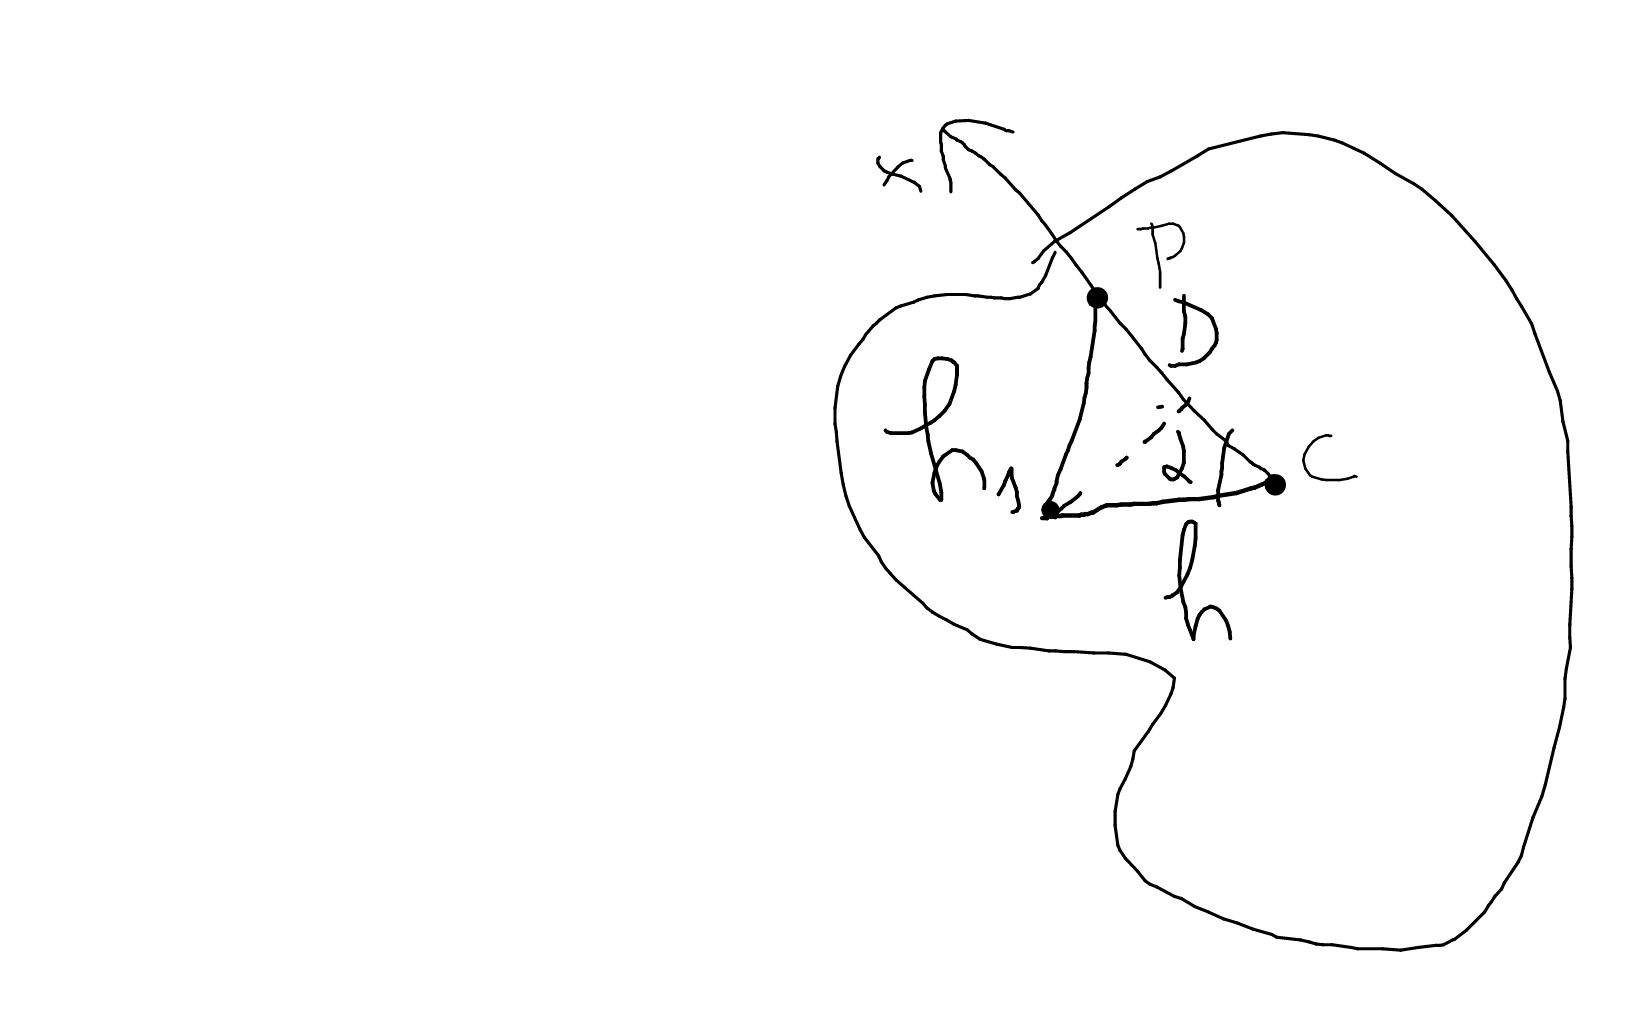
\includegraphics[width=0.5\textwidth]{TeoremaSteiner.png}
    \caption{Sezione del Corpo Rigido perpendicolare agli assi}
    \label{SezioneSteiner}
\end{figure}
Dove P è un punto appartenente alla sezione del corpo rigido, Q è un punto (del piano) dell'asse bb' e C è il centro di massa (che appartiene all'asse aa'). Scelto l'asse x passante per il punto P, notiamo che $h\cos\alpha$ è la componente di $\r_Q$ nel sistema solidale al corpo rigido e centrato in C. Essendo poi i due assi paralleli le distanze tra i punti C ed H sono costanti, quindi le considerazioni fatte sono equivalenti lungo tutte le sezioni del corpo rigido.
Calcolando il momento d'inerzia del corpo rigido rispetto all'asse bb' otteniamo:
\begin{equation}
\begin{split}
    I&=\int_Mh_1^2\dif m=\int_M(h^2+D^2-2hD\cos\alpha)\dif m=\\
    &=\int_Mh^2\dif m+\int_D^2M\dif m-2\int_MhD\cos\alpha\dif m=\\
    &=I_{aa'}+D^2\int_M\dif m-2D\int_Mh\cos\alpha\dif m=\\
    &=I_{aa'}+MD^2
\end{split}
\end{equation}
\note $\int_Mh\cos\alpha\dif m=\int_Mx\dif m=Mx_C=0$ per definizione di centro di massa e per il sistema di riferimento scelto.
Abbiamo quindi dimostrato il teorema di Steiner.
\end{thm}
\subsection{Rotazione del Corpo Rigido - 16 Maggio (S)}
\paragraph{Il Moto Rotatorio di un Corpo Rigido}
Consideriamo un corpo rigido che ruota attorno ad un certo asse $\va{\omega}$ e un sistema solidale al corpo rigido centrato nel centro di massa. Proiettando la velocità di un generico punto del corpo e del centro di massa lungo le direzioni parallele e perpendicolari a $\va{\omega}$ otteniamo:
\[\v_P=\v_{\parallel}+\v_\perp\quad\v_{O'}=\v_{O'\parallel}+\v_{O'\perp}\]
Da cui:
\begin{equation}
\begin{cases}
\v_{\parallel}=\v_{O'\parallel}\\
\v_{\perp}=\v_{O'\perp}+\va{\omega}\times\r'
\end{cases}
\end{equation}
Ossia se $\v_{O'\perp}=0$ allora la velocità perpendicolare del punto del corpo rigido coincide con la velocità rotazionale intorno al centro di massa e quindi il centro di massa appartiene all'asse istantaneo di rotazione, che è l'insieme dei punti che risolvono l'equazione $\v_{\perp}=\va{\omega}\times\r'$. Inoltre se $\r'$ è soluzione anche $\r_1'=k\omega+\r'$ lo è.
Quando si verifica la condizione citata si parla di \textbf{atto di moto elicoidale}, dove lo spostamento infinitesimo $\dif\r$ vale:
\begin{equation}
    \dif\r=\v_{\parallel}\dif t+(\va{\omega}\dif t\times\r')=\v_{\parallel}\dif t+(\dif\phi\times\r')
\end{equation}
\paragraph{Il I Teorema di Konig per i Corpi Rigidi}
\begin{equation}
\begin{split}
    \L_O&=\int_M\r\times\v\dif m=\int_M\left[(\r_C+\r')\times(\v_C+\v')\right]\dif m=\\
    &=\int_M\r_C\times\v_C\dif m+\int_M\r_C\times\v'\dif m+\int_M\r'\times\v_C\dif m+\int_M\r'\times\v'\dif m=\\
    &=\L_{CM}+\int_M\r_C\times\va{\omega}\times\r'\dif m+\left(\int_M\r'\dif m\right)\times\v_C+\int_M\r'\times\omega\times\r'\dif m=\\
    &=\L_{CM}+\int_M\r'\times\omega\times\r'\dif m=\L_C+\L_C'
\end{split}
\end{equation}
\note 
\[\L_C=\int_M\r'\times\v\dif m=\int_M\r'\times\v_C\dif m+\int_M\r'\times\va{\omega}\times\r'\dif m=\L_C'\]
Come avevamo già visto nel caso di un sistema di corpi a masse concentrate.\\

Consideriamo ora il caso di un corpo rigido che ruota attorno ad un asse sempre parallelo a se stesso. Scegliamo un sistema di riferimento cartesiano tale che:
\[\va{\omega}=\omega_z(t)\vu{k}=\omega(t)\k\]
Proiettiamo ora il momento angolare (calcolato usando il centro di massa come polo) lungo tale asse ricordando l'osservazione appena fatta:
\begin{equation}
\begin{split}
    \left(L_C\right)_z&=\L_C\cdot\k=\int_M\left[\r'\times\omega\times\r'\right]\cdot\k\dif m=\\
    &=\omega(t)\int_M\left[\r'\times\k\times\r'\right]\cdot\k\dif m=\\
    &=\omega(t)\int_M\left[\k\times\r'\right]\cdot(\k\times\r')\dif m=\\
    &=\omega(t)\int_M|\k\times\r'|^2\dif m=\omega(t)\int_M|\r'|^2\sin^2\alpha\dif m=\omega(t)\int_Mh^2\dif m=I_{zz}^C\omega(t)
\end{split}
\end{equation}
Ossia:
\[\boxed{(L_C)_z=I_{zz}^C\omega(t)}\]
Dove zz è l'asse di rotazione istantaneo, ossia l'asse z solidale al corpo rigido. Possiamo generalizzare questa considerazione spostando il polo ad un qualunque punto dell'asse ricordando la Formula di Steiner:
\begin{equation}
\begin{split}
    (L_\Omega)_z&=\L_\Omega\cdot\k=\omega(t)\int_M|\k\times\r'|^2\dif m=\omega(t)I_{zz}^\Omega\then\\
    &\then \boxed{(L_\Omega)_z=(I_{zz}^C+MD^2)\omega(t)}
\end{split}
\end{equation}
\note Usando la II cardinale attorno al centro di massa osserviamo che:
\[\dv{L_C}{t}=\M_C^{(e)}\then (M_C)_z=\dv{I_{zz}\omega}{t}=I_{zz}\dot{\omega}\]

\subsubsection{Casi Particolari di Rotazione}
\paragraph{Corpo Girevole attorno ad un Asse Fisso}
Un caso particolare di questa situazione è quella del \textbf{Pendolo Fisico} per cui possiamo applicare il caso generale della II Cardinale:
\[\dv{(L_\Omega)_z}{t}=I\dot{\omega}=(M_\Omega)_z-(\v_\Omega\times\P)_z=(M_\Omega)_z\]
\note $\v_\Omega=0$ in quanto l'asse è fisso per ipotesi. Inoltre risulta sufficiente il grado di libertà rotazionale per descrivere completamente il corpo rigido.

\paragraph{La Ruota - Cilindro Omogeneo che Ruota attorno al proprio asse di Simmetria}
Consideriamo una ruota che si muove senza sbandare parallelamente ad $\va{\omega}$ e senza sterzare. Il polo preferenziale a cui applicare la II Cardinale lungo l'asse di rotazione è il centro di Massa. 
Il moto della Ruota si riduce a \textbf{puro rotolamento} nel caso in cui l'asse istantaneo coincide con l'insieme di punti di contatto. La condizione di Rotolamento (per il quale l'attrito statico è nullo e quindi il lavoro dissipativo è nullo) è la seguente:
\[\v_\Omega(t)=0\iff \v_c=\va{\omega}\times\va{\Omega C}\then(v_C)_x=\overline{\Omega C}_y\omega_z-\overline{\Omega C}_zy=\overline{\Omega C}_y\omega_z=-R\omega\then\boxed{(v_C)_x=-R\omega}\]

\paragraph{Pendolo Fisico}
\begin{figure}[H]
    \centering
    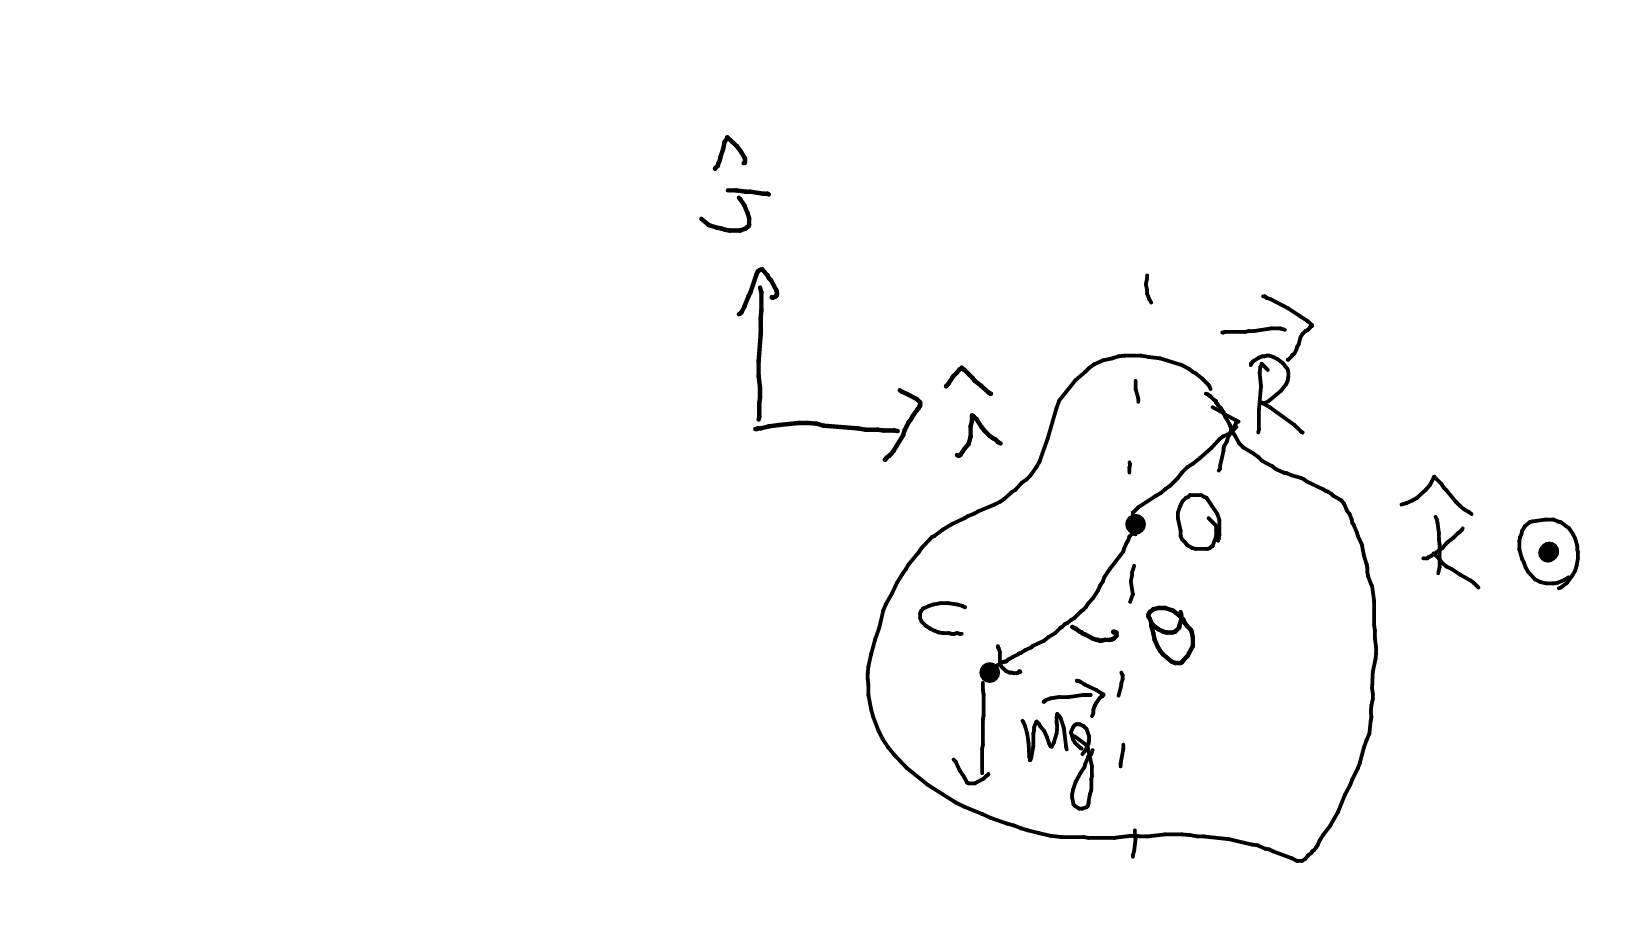
\includegraphics[width=0.5\textwidth]{PendoloFisico.png}
    \caption{Schema del Pendolo Fisico}
    \label{PendoloFisico}
\end{figure}
Consideriamo come in figura un corpo che può ruotare liberamente attorno ad un asse fisso. Scelto il punto O dell'asse (di una sezione perpendicolare all'asse di rotazione che include la verticale e il centro di massa C) come centro di riferimento e polo del momento possiamo calcolarlo come segue e poi proiettarlo lungo $\k$:
\[\M_O=\r_C\times M\va{g}+\r_O\times\R=\r_C\times M\va{g}\then (M_O)_z=-dMg\sin\theta=I\dot{\omega}=I\ddot{\theta}\]
Dove d è la distanza tra il polo e il centro di massa e $\theta$ è l'angolo d'inclinazione.
Otteniamo quindi la seguente equazione differenziale:
\[\boxed{\ddot{\theta}+\frac{Mgd}{I}\sin\theta=0}\]
Ossia l'\textbf{equazione del moto del pendolo fisico} che si riduce al pendolo semplice con $I=Md^2$.
\section{Termodinamica}
\subsection{Termodinamica - Introduzione}
Lo studio della termodinamica si basa sulla possibilità di raggiungere un'equilibrio, enunciata dal \textbf{principio zero}. Gli equilibri termodinamici compongono uno \textbf{spazio termodinamico} descritto da un certo numero di variabili (dette \textbf{grandezze termodinamiche}), tra le quali:
\begin{enumerate}
    \item Pressione
    \item Temperatura
    \item Volume
    \item Energia Interna
    \item Entropia
\end{enumerate}
\begin{defn}[Equilibrio Termodinamico]
L'equilibrio di un sistema termodinamico è costituito da tre equilibri che il sistema deve raggiungere:
\begin{enumerate}
    \item \textbf{Equilibrio Meccanico}, a cui corrisponde l'assenza di movimento macroscopico ed è caratterizzato dalla pressione, si raggiunge quando la pressione esterna è uguale a quella interna.
    \item \textbf{Equilibrio Chimico}, a cui corrisponde l'assenza di reazioni chimiche e trasformazioni di fase, a cui corrisponde il potenziale chimico, si raggiunge quando il potenziale chimico dei reagienti $\mu_A$ è uguale a quello dei prodotti $\mu_B$.
    \item \textbf{Equilibrio Termico}, quando la temperatura dell'ambiente e quella del sistema sono le stesse.
\end{enumerate}
\end{defn}
Queste tre grandezze sono \textbf{intensive} in quanto non dipendono dalle dimensioni del sistema. Le grandezze che dipendono dalle dimensioni sono dette \textbf{estensive} (additive) e includono massa, volume, entropia ed energia interna.
L'equazione di stato di un sistema termodinamico è un'equazione del tipo:
\[t=t(p,V)\quad p=p(t,V)\]
Ossia una relazione tra pressione, volume e temperatura.
\begin{defn}[Varianza]
La varianza di un sistema termodinamico corrisponde al numero di gradi di libertà di quel sistema, ossia il numero di grandezze necessario a descriverlo. 
\end{defn}
Utilizzando la \textbf{Regola di Gibbs} possiamo calcolare la varianza di un sistema come segue:
\begin{equation}
    \boxed{v=n-f+2}
\end{equation}
Dove n è il numero di componenti (sostanze) ed f il numero di fasi. Quando $v=0$ il sistema si trova nel suo \textbf{punto triplo}, ossia un punto particolare dello spazio termodinamico determinato da specifiche coordinate di volume, pressione e temperatura. 

\subsection{Primo Principio della Termodinamica - 30 Maggio (S)}
Consideriamo la quantità di calore infinitesima fornita ad un corpo che non sta subendo cambiamenti di fase, possiamo definire la grandezza \textbf{capacità termica} come:
\[C=\dv{Q}{t}\quad\dif t\neq 0\]
Si osserva empiricamente che tale grandezza è proporzionale alla massa e quindi al numero di moli secondo una costante detto \textbf{calore specifico} (di una sostanza) o calore specifico molare rispettivamente:
\[C=mc=n\overline{c}\]
Inoltre possiamo definire il \textbf{calore latente} per un sistema che sta subendo un cambiamento di fase:
\[\lambda=\dv{Q}{m}\]\\
Parliamo di \textbf{trasformazione termodinamica} da uno stato iniziale ad uno stato finale un passaggio da un'equilibrio termodinamico ad un altro. In generale tale trasformazione risulta impossibile da rappresentare su un piano termodinamico p-V in quanto solo agli equilibri le grandezze termodinamiche sono ben definite. Possiamo però rappresentare come segue una trasformazione di questo tipo:
\begin{figure}[H]
    \centering
    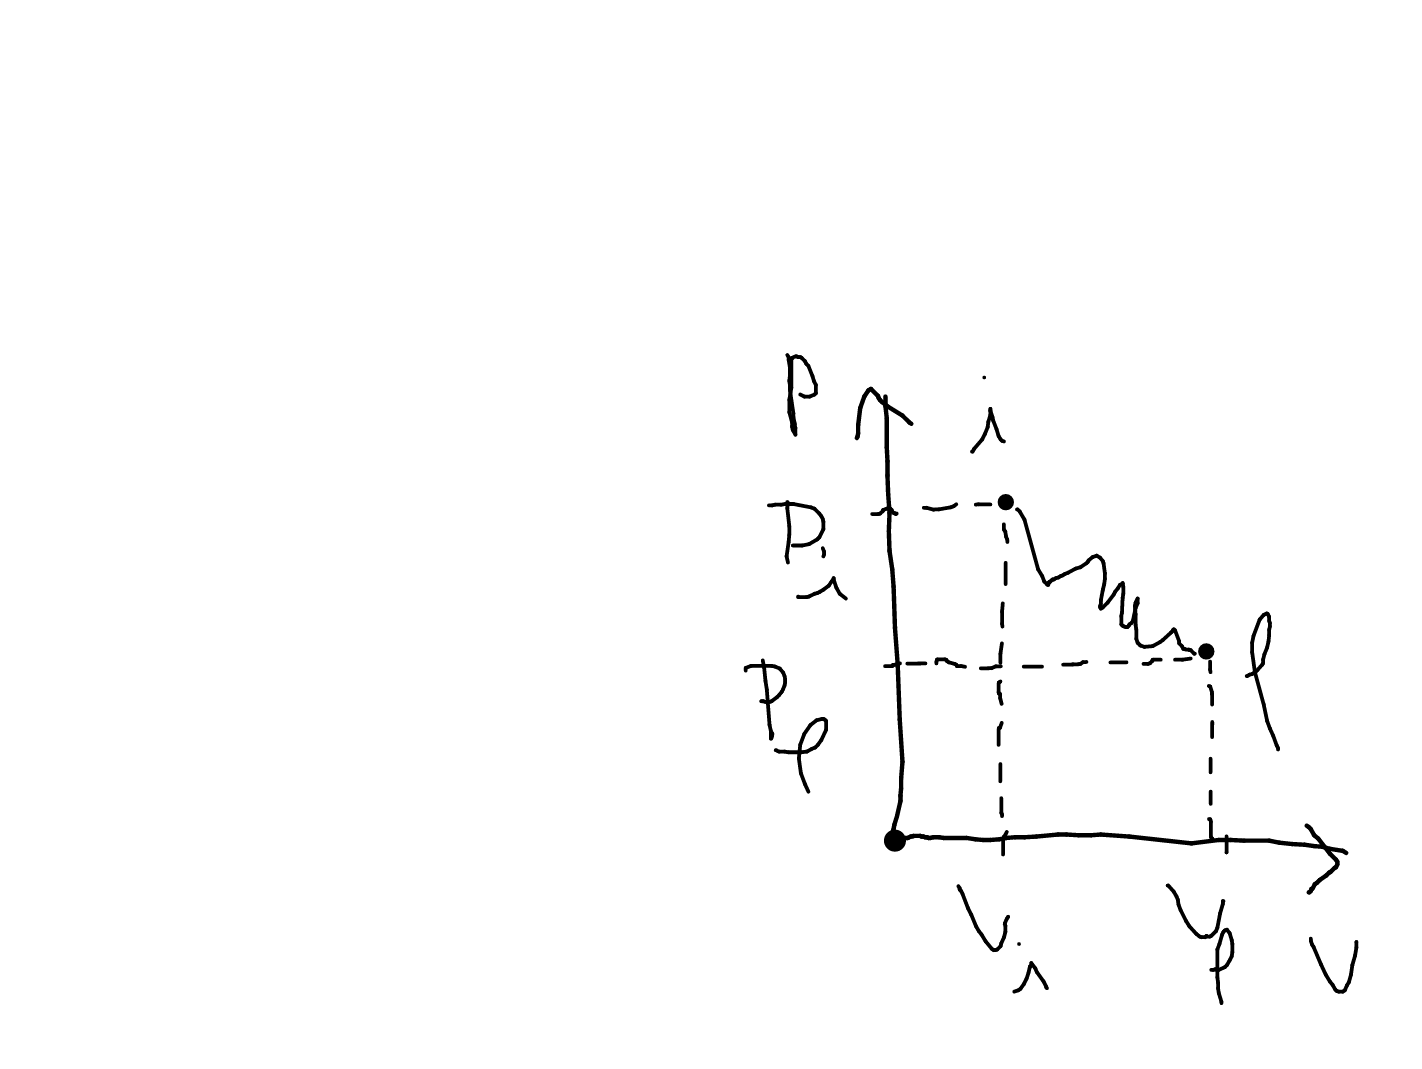
\includegraphics[width=0.5\textwidth]{TrasformazioneIrreversibile.png}
    \caption{Esempio di Trasformazione Termodinamica}
    \label{TrasfIrrev}
\end{figure}
Possiamo quindi formulare il \textbf{Primo Principio della Termodinamica} come segue: la variazione di \textbf{energia interna} è la differenza tra il calore scambiato con l'esterno e il lavoro compiuto (o subito) dal sistema.
\begin{equation}
    \boxed{Q-L=\Delta U}
\end{equation}
\paragraph{Trasformazioni Infinitesime}
Queste sono trasformazioni ottenute per infinitesime quantità di calore e lavoro scambiati con l'esterno da un sistema (a cui corrispondono infinitesima variazioni di pressione, volume e temperatura). Studiando un sistema con varianza 2 otteniamo il primo principio per quantità infinitesima:
\[\delta Q-\delta L=\dif U\]
Notiamo che Q ed L sono forme differenziali in quanto non sono funzioni di stato, diversamente dall'energia interna. Calcoliamo la quantità di calore infinitesima fornita utilizzando la definizione di lavoro e la proprietà di differenziale esatto di energia interna:
\[\delta Q=\dif U+\delta L=\left(\pdv{U}{t}\right)_V\dif t+\left(\pdv{U}{V}\right)_t\dif V+p^{(e)}\dif V\]
Otteniamo quindi la seguente \textbf{formula del calore} per trasformazioni infinitesime:
\begin{equation}
\boxed{\delta Q=\left(\pdv{U}{t}\right)_V\dif t+\left[\left(\pdv{U}{V}\right)_t+p^{(e)}\right]\dif V}
\end{equation}
Per una trasformazione infinitesima \textbf{isocora} si riduce a:
\[\delta Q=\left(\pdv{U}{t}\right)_V\dif t\]
Ma per definizione di calore specifico molare:
\[\dv{Q}{t}=\left(\pdv{U}{t}\right)_V=n\overline{c}_V\then \boxed{\delta Q=n\overline{c}_V\dif t+\left[\left(\pdv{U}{V}\right)_t+p^{(e)}\right]\dif V}\]
Siccome l'energia interna è una funzione di stato, questa espressione è valida per ogni trasformazione infinitesima.
Per i liquidi e i solidi, considerati incompressibili possiamo porre $\dif V=0$, mentre il calore specifico molare è uguale sia a pressione che a volume costante. Pertanto il calore si riduce all'espressione della trasformazione isocora per liquidi e solidi.
\subsubsection{Le Leggi dei Gas Ideali}
Per quanto riguarda i gas il comportamento si può generalizzare ad ogni gas nel caso in cui essi siano \textbf{rarefatti}, ossia poco densi e ad alta temperatura. In particolare valgono le seguenti leggi:
\begin{enumerate}
    \item La Prima Legge di Gay-Lussac \[V=V_0(1+\alpha t)\]
    Dove $\alpha$ è una costante che vale $\frac{1}{273,16^\circ C}$ per gas rarefatti, $V_0$ è il volume a pressione atmosferica e $0^\circ C$ e la pressione è costante.
    \item La Seconda Legge di Gay-Lussac \[p=p_0(1+\alpha t)\]
    Con volume costante e dove $p_0$ è la costante atmosferica.
    \item La Legge di Boyle \[pV=p_0V_0\]
    Che è valida a temperatura costante.
\end{enumerate}
Da queste leggi possiamo ricavare l'\textbf{equazione di stato} per i gas ideali. Immaginiamo di sottoporre il gas ad una trasformazione isobara, vale allora la prima legge di Gay-Lussac:
\[V_1=V_0(1+\alpha t)\]
Sottoponiamola poi ad una trasformazione isoterma, in modo che sia valida la legge di Boyle:
\[pV=p_0V_1=p_0V_0(1+\alpha t)\]
Esplicitando $V_0$ come prodotto del numero di moli e del volume molare otteniamo (abbiamo implicitamente usato la \textbf{Legge di Avogadro} nell'affermare che tutti i gas rarefatti hanno lo stesso volume molare):
\[pV=p_0n\overline{v}_0\alpha \left(t+\frac{1}{\alpha}\right)\]
Definiamo quindi una nuova scala di temperatura, detta \textbf{scala di Kelvin} tale che $\theta=(t+273,16)K$ e poi definiamo la \textbf{costante universale dei gas} come $R=p_0\overline{v}_0\alpha$ ottenendo infine:
\begin{equation}
\boxed{pV=nR\theta}
\end{equation}
Ossia l'equazione di stato dei gas perfetti.

\subsubsection{Il II Esperimento di Joule}
\begin{figure}[H]
    \centering
    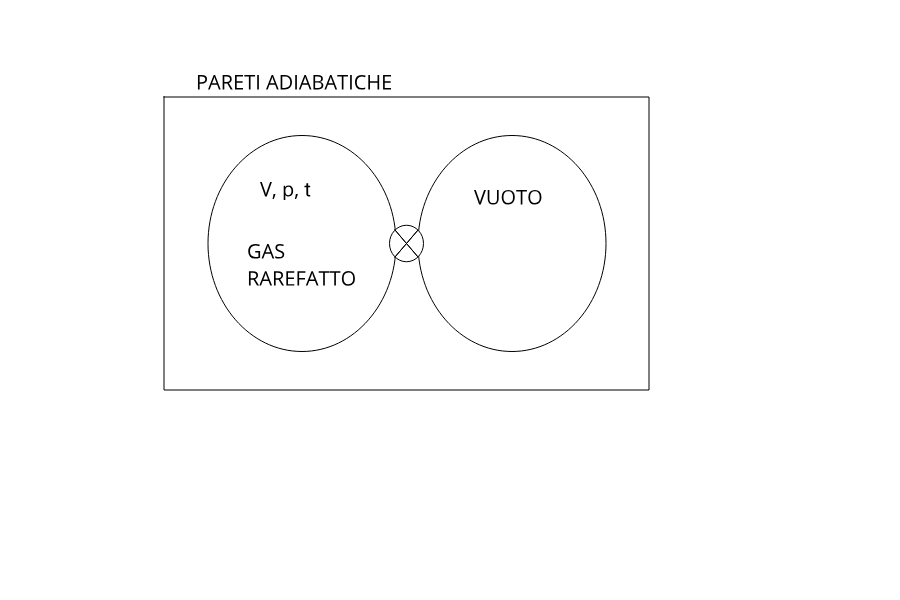
\includegraphics[width=0.5\textwidth]{SecondoJoule.png}
    \caption{Stato Iniziale del Secondo Esperimento di Joule}
    \label{SecondoJoule}
\end{figure}
Costruiamo un sistema isolato con delle pareti adiabatiche dall'esterno e in contatto con un altro contenitore tramite una valvola. Immaginiamo di \textbf{bruscamente} aprire questa valvola, otterremo che all'equilibrio il gas occupa tutto il volume. Inoltre si può misurare che all'equilibrio la temperatura risulta invariata:\\
\begin{center}
\begin{tabular}{c|c|c|c}
    INIZIO & $V_i=V_1$ & $p_i=p_0$ & $t_i=t_1$ \\
    \hline
    FINE & $V_f=V_1+V_2$ & // & $t_f=t_1$
\end{tabular} 
\end{center}
Ripetendo l'esperimento a densità molare decrescente otteniamo il seguente grafico:\\
\begin{center}
\begin{tikzpicture}
\begin{axis}[
    axis lines = left,
    xlabel = $\frac{n}{V_i}$,
    ylabel = {$t_i-t_f$},
]
\addplot [
    domain=0:10, 
    samples=10, 
    color=red,
]
{x*0.3};
\end{axis}
\end{tikzpicture}
\end{center}
Ossia otteniamo una funzione che tende a 0 al calare della densità molare. Osserviamo inoltre che essendo le pareti adiabatiche e fisse, esse isolano il sistema sia meccanicamente che termicamente in modo che non ci siano scambi di calore nè l'ambiente possa compiere lavoro sul sistema (o viceversa), quindi la variazione di energia interna è nulla:
\[\Delta U=Q-L=0\then U_i=U_f\]
Scelte t e V come variabili termodinamiche del sistema allora vale:
\[U(t_1,V_1)=U(t_1,V_1+V_2)=U(t_1,yV_1)\]
Ossia il volume a temperatura costante varia linearmente, quindi:
\[\pdv{U}{V}=0\then U=U(t)=U(\theta)\]
Ossia l'energia interna è una \textbf{funzione di stato} che dipende unicamente dalla \textit{temperatura}.\\
Pertanto un gas ideale è descritto termodinamicamente dall'equazione di stato e della funzione energia interna:
\begin{equation}
\begin{cases}
pV=nR\theta\\
U=U(\theta)
\end{cases}
\end{equation}
Per un gas ideale vale allora la seguente espressione di calore ed energia interna:
\begin{equation}
\boxed{(\delta Q)_V=n\overline{c}_V\dif\theta=\dif U}\then \boxed{U(\theta)=\int n\overline{c}_V(\theta)\dif\theta+cost}
\end{equation}
Queste considerazioni (fatte in questa situazione) sono tuttavia valide in ogni trasformazione termodinamica, in quanto l'energia interna è una funzione di stato. Mentre l'espressione generale del calore è:
\[\delta Q=n\overline{c}_V\dif\theta+p^{(e)}\dif V\]
\paragraph{Calore Specifico Molare}
Il calore specifico molare a volume costante per i gas si comporta (sommariamente) come in figura, dove i monoatomici hanno $\overline{c}_V$ costante, i biatomici hanno $\overline{c}_V$ a "scaletti" a cui corrisponde microscopicamente lo "sblocco" dei gradi di libertà delle molecole e infini i poliatomici hanno andamenti altamente complicati, la cui curva tende a diventare più \textit{liscia} all'aumentare degli atomi componenti. Generalmente la fascia considerata è quella in cui i gas biatomici hanno $\overline{c}_V=\frac{5}{2}R$ e i monoatomici hanno $\overline{c}_V=\frac{3}{2}R$.\\
Vale inoltre la \textbf{legge di Mayer} che stabilisce che:
\begin{equation}
\boxed{\overline{c}_p-\overline{c}_V=R}
\end{equation}

\subsection{Le Trasformazioni Reversibili - 1 Giugno (S)}
\begin{defn}[Trasformazione Quasistatica]
Si definisce trasformazione \textbf{quasistatica} una trasformazione ottenuta tramite somma di trasformazioni infinitesime. Praticamente ciò implica che una trasformazione quasistatica si può rappresentare sul piano p-V:
\[\int_A^B\delta Q-\int_A^B\delta L=\int_A^B\dif U\]
In questo caso sono ben definite tutte le grandezze termodinamiche per ogni variazione allora per il calcolo del lavoro possiamo utilizzare la pressione del gas (uguale a quella esterna). 
\end{defn}
\begin{defn}[Trasformazione Reversibile]
Una trasformazione quasistatica si dice reversibile se può essere ripetuta in senso inverso seguendo gli stessi stati di equilibrio punto per punto. 
\end{defn}
Tra le più comuni trasformazioni reversibili individuiamo le seguenti quattro:
\begin{figure}[H]
    \centering
    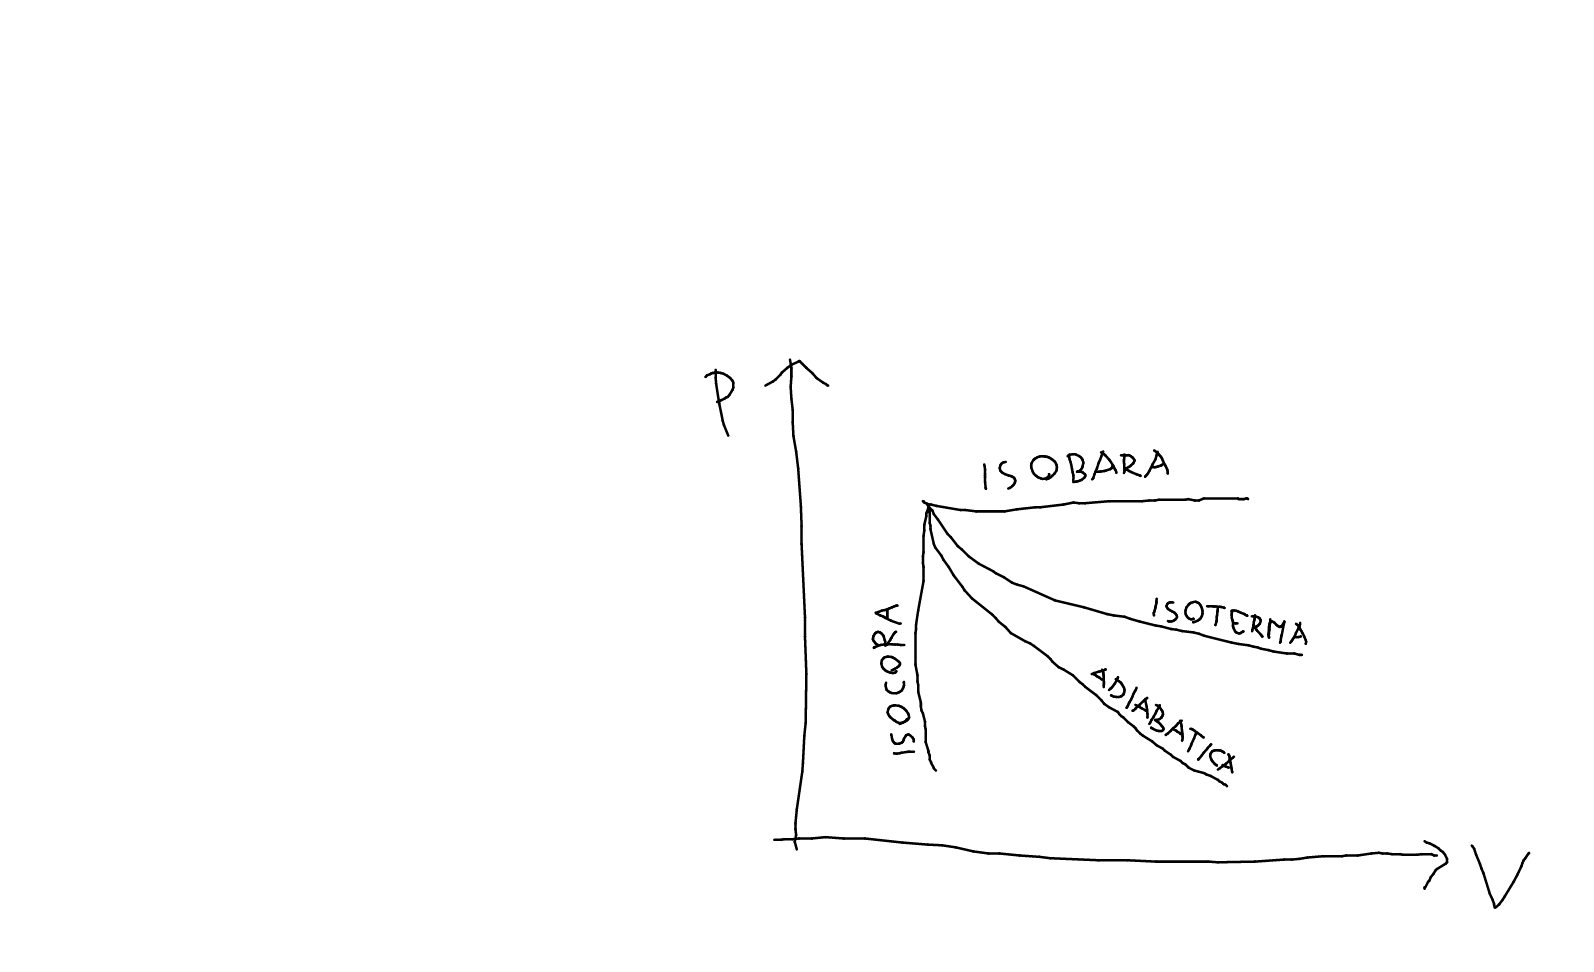
\includegraphics[width=0.6\textwidth]{TrasformazioniReversibili.png}
    \caption{Le Maggiori Trasformazioni Reversibili }
    \label{TrasfRevers}
\end{figure}
\paragraph{Trasformazione Adiabatica Reversibile} Considerando un'adiabatica reversibile possiamo applicare il primo principio per le trasformazioni infinitesime e poi integrando tra uno stato A e B:
\[\delta Q=\dif U+\delta L=n\overline{c}_V\dif\theta+p\dif V=0\then \overline{c}_V\frac{\dif\theta}{\theta}+R\frac{\dif V}{V}=0\then \overline{c}_V\ln\frac{\theta_B}{\theta_A}+R\ln\frac{V_B}{V_A}=0\]
Definita la costante $\gamma=\frac{\overline{c}_p}{\overline{c}_V}$ allora possiamo esplicitare come segue:
\begin{equation}
\begin{split}
    \ln\frac{\theta_B}{\theta_A}+\frac{R}{\overline{c}_V}\ln\frac{V_B}{V_A}&=0\\
    \ln\frac{\theta_B}{\theta_A}+(\gamma-1)\ln\frac{V_B}{V_A}&=0\\
    \ln\frac{\theta_B}{\theta_A}+\ln\left(\frac{V_B}{V_A}\right)^{\gamma-1}&=0\\
    \ln\left[\frac{\theta_B}{\theta_A}\left(\frac{V_B}{V_A}\right)^{\gamma-1}\right]&=0\\
\end{split}
\end{equation}
Per le proprietà dei logaritmi otteniamo:
\[\frac{\theta_B}{\theta_A}\left(\frac{V_B}{V_A}\right)^{\gamma-1}=1\then \theta_BV_B^{\gamma-1}=\theta_AV_A^{\gamma-1}\]
Ossia:
\begin{equation}
\boxed{\theta V^{\gamma-1}=cost}
\end{equation}
Utilizzando l'equazione di stato dei gas ideali possiamo anche ottenere le seguenti espressioni:
\[pV^{\gamma}=cost\quad Tp^{\frac{1-\gamma}{\gamma}}\]

\subsubsection{Secondo Principio della Termodinamica}
\begin{defn}[Sorgente]
Un sistema che mantiene la propria temperatura costante.
\end{defn}
\begin{defn}[Enunciato di Clausius]
Non è possibile effettuare una trasformazione termodinamica il cui unico risultato sia il trasferimento di una quantità finita di calore da una sorgente fredda ad una calda.
\end{defn}
\begin{defn}[Enunciato di Kelvin-Planck]
Non è possibile realizzare una trasformazione termodinamica che abbia come unico risultato la trasformazione in lavoro del calore fornito da una sorgente.
\end{defn}
\begin{defn}[Rendimento]
Il rendimento di una macchina termica si definisce come:
\[\eta=\frac{L}{Q_A}=1+\frac{Q_B}{Q_A}\]
\end{defn}
\note L'enunciato di Kelvin equivale a dire che il rendimento di una macchina termica è minore di 1.\\
Dimostriamo ora l'equivalenza di questi due enunciati.
\begin{thm}[Clausius Implica Kelvin]
Supponiamo per assurdo che l'enunciato di Kelvin sia falso. Possiamo quindi costruire una macchina termica K che converte interamente lavoro in calore (ad esempio il Mulinello di Joule). Introduciamo poi un'altra macchina frigorifera $M_f$ su cui la prima macchina compie lavoro in modo che assorba calore dalla prima sorgente e ceda calore ad un'altra sorgente, più calda. L'effetto totale è quindi che la sorgente a temperatura fredda ha ceduto calore ad una sorgente a temperatura più alta. Ciò implica che l'enunciato di Clausius sia falso, abbiamo quindi raggiunto l'assurdo.
\begin{figure}[H]
    \centering
    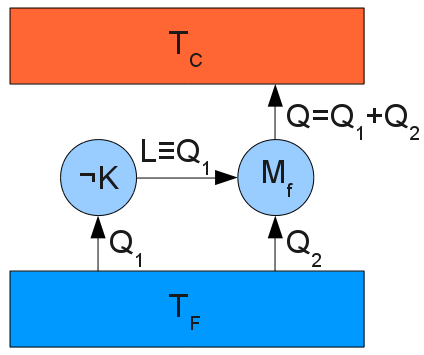
\includegraphics[width=0.5\textwidth]{Kelvin_dimostrazione_assurdo.png}
    \caption{Schema del Sistema Costruito}
    \label{ClausiusKelvin}
\end{figure}
\end{thm}
\begin{thm}[Kelvin Implica Clausius]
Supponiamo per assurdo che l'enunciato di Clausius sia falso. Costruiamo quindi una macchina termica C che assorbe una quantità di calore Q da una sorgente fredda e lo cede ad una calda (in quanto Clausius è falso) come unico risultato. Introduciamo quindi una macchina termica $M_t$ che assorbe una quantità di calore Q' compiendo lavoro L in modo che la quantità di calore ceduta alla sorgente a temperatura minore sia la stessa di quella assorbita dalla macchina C. Abbiamo quindi costruito una trasformazione il cui unico risultato sia quello di convertire calore in lavoro (l'effetto totale è di non coinvolgere la sorgente a temperatura fredda), quindi l'enunciato di Kelvin è falso. Abbiamo raggiunto l'assurdo, come volevasi dimostrare. 
\begin{figure}[H]
    \centering
    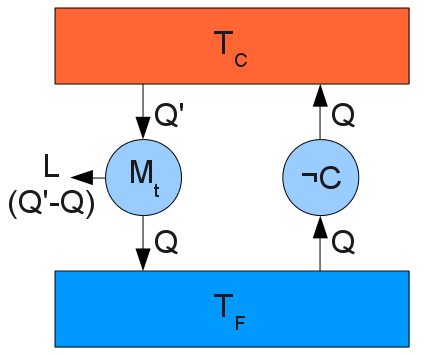
\includegraphics[width=0.5\textwidth]{Clausius_dimostrazione_assurdo.png}
    \caption{Schema del Sistema Costruito}
    \label{KelvinClausius}
\end{figure}
\end{thm}

\paragraph{Teorema di Carnot}
\begin{thm}[Teorema di Carnot]
Ogni macchina reversibile che lavoro tra due sorgenti alla stessa temperatura ha lo stesso rendimento. Qualsiasi altra macchina che lavori tra queste sorgenti ha rendimento non maggiore. Il risultato è indipendente dalle trasformazioni del ciclo. 
\end{thm}
\begin{proof}
Costruiamo due macchine termiche X ed R che lavorano tra le stesse sorgenti e tali da compiere lo stesso lavoro L, assorbendo rispettivamente una quantità di calore $Q_1$ e $Q_1'$ e cedendo una quantità di calore $Q_2$ e $Q_2'$ alla sorgente calda e fredda rispettivamente. 
\begin{figure}[H]
    \centering
    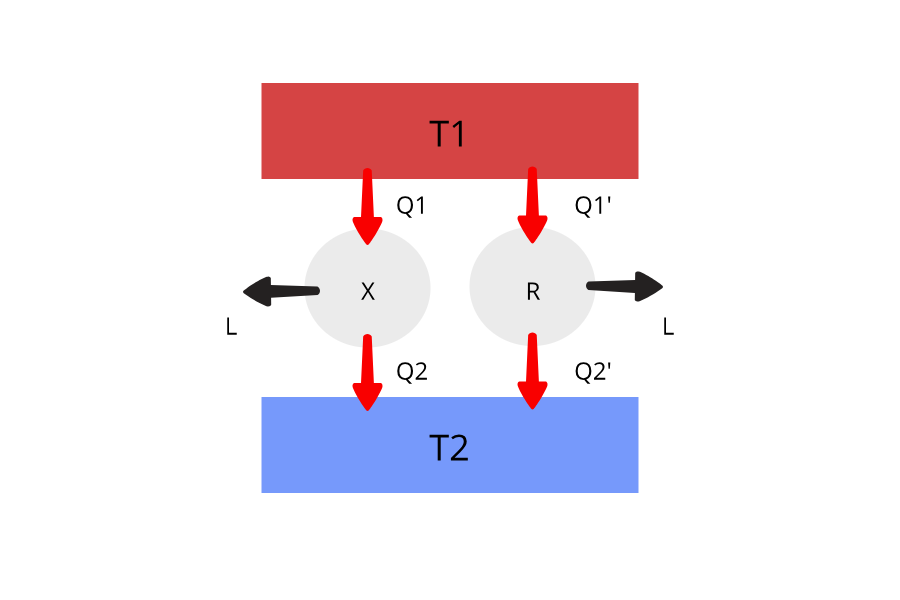
\includegraphics[width=0.7\textwidth]{TeoremaCarnot1.png}
    \label{TeoremaCarnot1}
\end{figure}
Supponendo che la macchina \textbf{R} sia reversibile, utilizziamo il lavoro della macchina \textbf{X} per invertire il ciclo della macchina R in modo che diventi refrigerante (stavolta i calore scambiati da R sono invertiti di segno).
\begin{figure}[H]
    \centering
    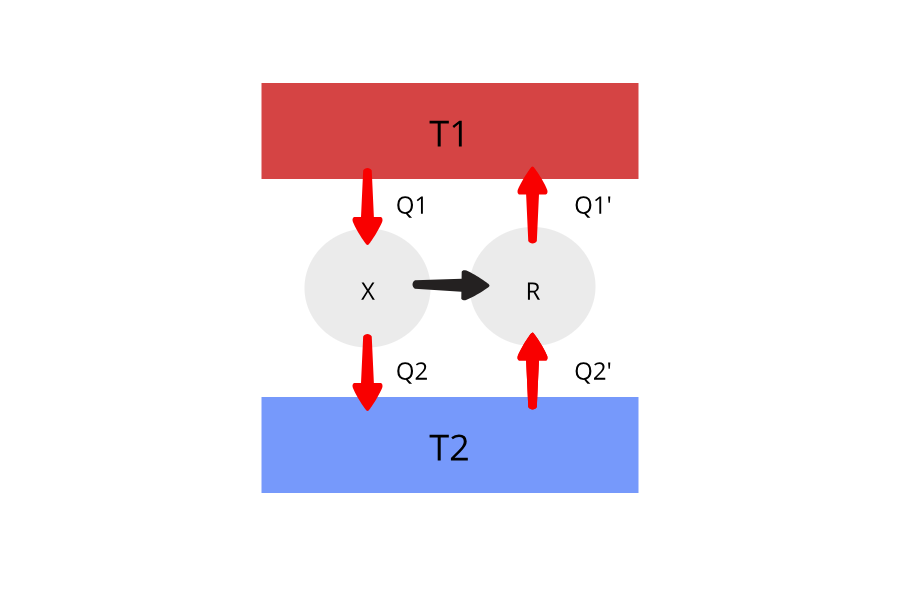
\includegraphics[width=0.7\textwidth]{TeoremaCarnot2.png}
    \label{TeoremaCarnot2}
\end{figure}

Per l'enunciato di Clausius deve risultare che la quantità di calore totale ceduta dalla sorgente calda è maggiore di quella ceduta da quella fredda, quindi otteniamo:
\[\abs{Q_1}\geq\abs{Q_1'}\then \frac{Q_1'}{Q_1}\leq 1\]
Calcoliamo quindi i rendimenti delle due macchine:
\begin{equation}
\eta_X=\frac{L}{Q_1}\quad\eta_R=\frac{L}{Q_1'}\then \eta_X\abs{Q_1}=\eta_R\abs{Q_1'}\then \eta_X=\eta_R\frac{\abs{
Q_1'}}{\abs{Q_1}} \leq \eta_R\then\boxed{\eta_X\leq\eta_R}
\end{equation}

Abbiamo dimostrato la \textbf{prima parte della tesi}. Dimostriamo ora la seconda.
Supponiamo che X sia reversibile, allora possiamo invertire i ragionamenti fatti in modo da ottenere:
\[\eta_X\geq\eta_R\]
Ma allora l'unica possibilità è che i due rendimenti coincidano:
\begin{equation}
\boxed{\eta_X=\eta_R}
\end{equation}
\end{proof}
\note Il risultato è indipendente dalle trasformazioni del ciclo in quanto l'unica proprietà che abbiamo assunto dalle macchine è che una fosse reversibile.\\
\note L'uguaglianza come caso limite nel primo risultato è nel caso in cui entrambe le macchine siano irreversibili oppure nel caso $Q_1=Q_1'=0\iff L=0$ ossia la macchina sta operando alcuna trasformazione.

\begin{prop}[Definizione di Temperatura Assoluta]
Dimostrato il Teorema di Carnot siamo in grado di dare una definizione assoluta di temperatura utilizzando il risultato per cui ogni macchina reversibile che opera tra certe due sorgenti ha lo stesso rendimento, ciò implica che il rendimento di una macchina reversibile R è funzione delle due temperature:
\[\eta=\eta(t_1,t_2)=1+\frac{Q_2}{Q_1}\]
Definiamo quindi la funzione g come segue:
\[g(t_1,t_2)=1-\eta(t_1,t_2)=\frac{\abs{Q_2}}{\abs{Q_1}}\]
Costruiamo poi il seguente sistema formato da tre sorgenti e due macchine termiche nel modo seguente (dove $\abs{Q_2}=\abs{Q_2'}$):
\begin{figure}[H]
    \centering
    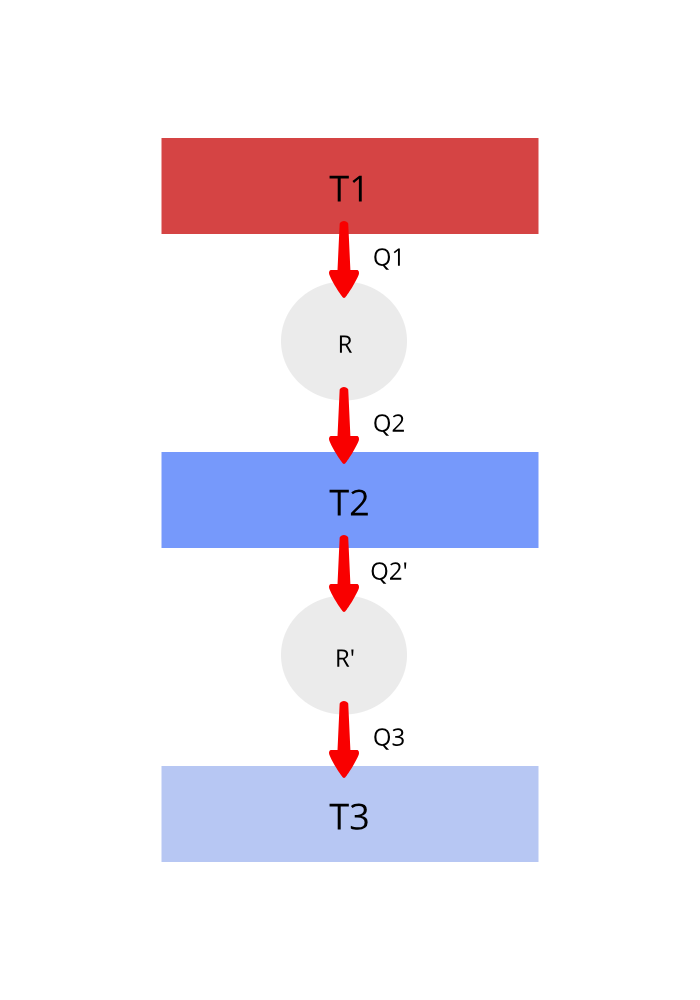
\includegraphics[width=0.4\textwidth]{TemperaturaAssoluta.png}
    \label{TeoremaCarnot2}
\end{figure}
Corto-circuitiamo le due macchine termiche in modo da ottenere un'unica macchina termica reversibile che lavora tra la sorgente a temperatura $t_1$ e quella a temperatura $t_3$ scambiando rispettivamente una quantità di calore $Q_1$ e $Q_3$.
\begin{figure}[H]
    \centering
    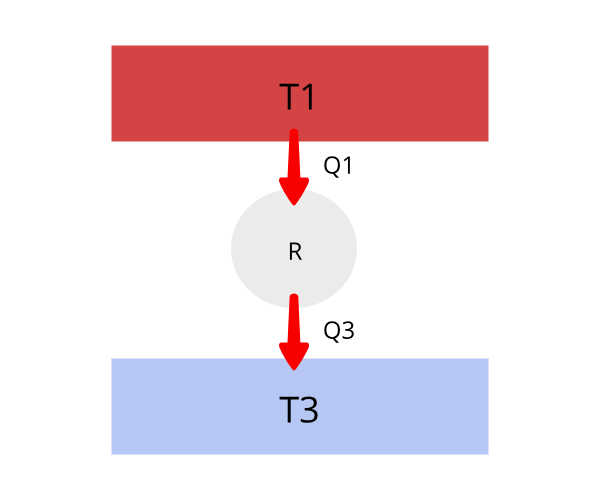
\includegraphics[width=0.5\textwidth]{TempAss.png}
\end{figure}
La funzione g di questa macchina termica è:
\[g(t_1,t_3)=\frac{\abs{Q_3}}{\abs{Q_1}}\]
Mentre delle due macchine singolarmente:
\[g(t_1,t_2)=\frac{\abs{Q_2}}{\abs{Q_1}}\quad g(t_2,t_3)=\frac{\abs{Q_3}}{\abs{Q_2'}}\]
Allora vale la relazione:
\[g(t_1,t_3)=g(t_1,t_2)\cdot g(t_2,t_3)\quad\forall t_2\]
Ciò significa che g è una funzione indipendente da $t_2$. Possiamo scriverla quindi come rapporto di una funzione f applicata in $t_3$ e applicata in $t_2$:
\[g(t_1,t_3)=\frac{f(t_3)}{f(t_1)}\]
Chiamiamo questa funzione f(t) \textbf{temperatura termodinamica assoluta} e poniamo $g(P.T.)=T_{pt}=273,16K$ ossia poniamo la temperatura assoluta del punto triplo (un punto termodinamico ben definito) dell'acqua uguale a $273,16K$. Possiamo quindi misurare la temperatura $T_x$ di una sorgente misurando i calori scambiati con una macchina che lavoro tra $T_{pt}$ e $T_x$:
\[T_x=T_{pt}\frac{\abs{Q_x}}{\abs{Q_{pt}}}\]
Ossia il II Principio fornisce un metodo di misurazione \textbf{assoluta} di temperatura.
\end{prop}
\note La scala assoluta e la scala Kelvin coincidono in quanto:
\[\frac{T_x}{T_{pt}}=\frac{\theta_x}{\theta_{pt}}=\frac{\theta_x}{T_{pt}}\iff T_x=\theta_x\]

\subsubsection{Il Ciclo di Carnot}
Il Ciclo di Carnot è un ciclo composto da quattro trasformazioni reversibili:
\begin{enumerate}
    \item AB \textbf{Espansione Isoterma} ($Q>0$)
    \item BC \textbf{Espansione Adiabatica} ($Q=0$)
    \item CD \textbf{Compressione Isoterma} ($Q<0$)
    \item DA \textbf{Compressione Adiabatica} ($Q=0$)
\end{enumerate}
\begin{figure}[H]
    \centering
    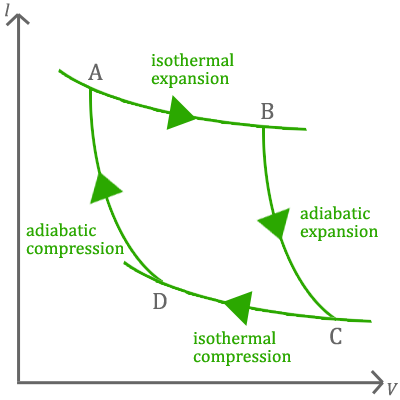
\includegraphics[width=0.6\textwidth]{CicloCarnot.png}
    \caption{Il Ciclo di Carnot}
    \label{CicloCarnot}
\end{figure}
Si può dimostrare che questa è l'unica trasformazione ciclica (percorsa nel senso in figura, tale che la macchina si comporti da macchina termica e \textit{compia} lavoro) che avviene solo tra due sorgenti (e quindi \textbf{due temperature}. Studiamo ora quanto vale il rendimento di una macchina (detta \textbf{macchina di Carnot}) che compie questo ciclo. \\
Durante l'espansione isoterma AB il calore è assorbito dalla sorgente calda a temperatura $T_2$ (uguale al lavoro compiuto dal sistema) e vale:
\[Q_2=nRT_1\ln\frac{V_B}{V_A}\]
Durante l'espansione adiabatica BC vale la relazione tra volume e temperatura:
\[T_BV_B^{\gamma-1}=T_CV_C^{\gamma-1}\iff T_2V_B^{\gamma-1}=T_1V_C^{\gamma-1}\then \left(\frac{V_C}{V_B}\right)^{\gamma-1}=\frac{T_2}{T_1}\]
Durante la compressione isoterma CD il calore ceduto:
\[Q_1=nRT_1\ln\frac{V_D}{V_C}\]
E infine dalla compressione adiabatica DA otteniamo:
\[T_DV_D^{\gamma-1}=T_AV_A^{\gamma-1}\iff T_1V_D^{\gamma-1}=T_2V_A^{\gamma-1}\then \left(\frac{V_D}{V_A}\right)^{\gamma-1}=\frac{T_2}{T_1}\]
Combinando le due equazioni ottenute dalle adiabatiche:
\[\left(\frac{V_C}{V_B}\right)^{\gamma-1}=\frac{T_2}{T_1}=\left(\frac{V_D}{V_A}\right)^{\gamma-1}\then \frac{V_C}{V_B}=\frac{V_D}{V_A}\then\boxed{\frac{V_C}{V_D}=\frac{V_B}{V_A}}\]
Il rendimento del ciclo vale 
\begin{equation}
\begin{split}
    \eta&=1+\frac{Q_1}{Q_2}=1+\frac{nRT_B\ln\frac{V_D}{V_C}}{nRT_A\ln\frac{V_B}{V_A}}=\\
    &=1+\frac{T_1\ln\frac{V_D}{V_C}}{T_2\ln\frac{V_B}{V_A}}=1-\frac{T_1\ln\frac{V_C}{V_D}}{T_2\ln\frac{V_B}{V_A}}=\\
    &=\boxed{1-\frac{T_1}{T_2}}
\end{split}
\end{equation}
Come volevasi dimostrare, il rendimento di una macchina di Carnot dipende unicamente dalle temperature delle \textit{due} sorgenti tra cui opera. Inoltre usando il \textbf{Teorema di Carnot} ricaviamo che una macchina qualunque che opera tra due sorgenti (e quindi compie lo stesso tipo di trasformazioni, anche se irreversibili) ha un rendimento:
\[\eta\leq1-\frac{T_1}{T_2}\]
Inoltre per definizione di rendimento:
\[\eta=1+\frac{Q_1}{Q_2}\then \frac{Q_1}{Q_2}\leq -\frac{T_1}{T_2}\then \boxed{\frac{Q_1}{T_1}+\frac{Q_2}{T_2}}\]
Questa disuguaglianza è particolarmente importante in quanto rappresenta una prima forma di enunciato per il secondo principio della termodinamica, ma deve essere generalizzato in quanto per trovare questo risultato abbia supposto due ipotesi:
\begin{enumerate}
    \item La trasformazione operata dalla macchina è \textbf{ciclica}
    \item La macchina termica opera tra \textbf{due sorgenti}
\end{enumerate}

\subsection{Disuguaglianza di Clausius ed Entropia - 6 Giugno (S)}
\begin{thm}[Teorema di Clausius]
Il Teorema di Clausius permette di generalizzare il risultato ottenuto ad un numero arbitrario di sorgenti (fino ad una continuità di sorgenti). Consideriamo prima di tutto una macchina termica che compie una trasformazione ciclica tra n sorgenti:
\begin{figure}[H]
    \centering
    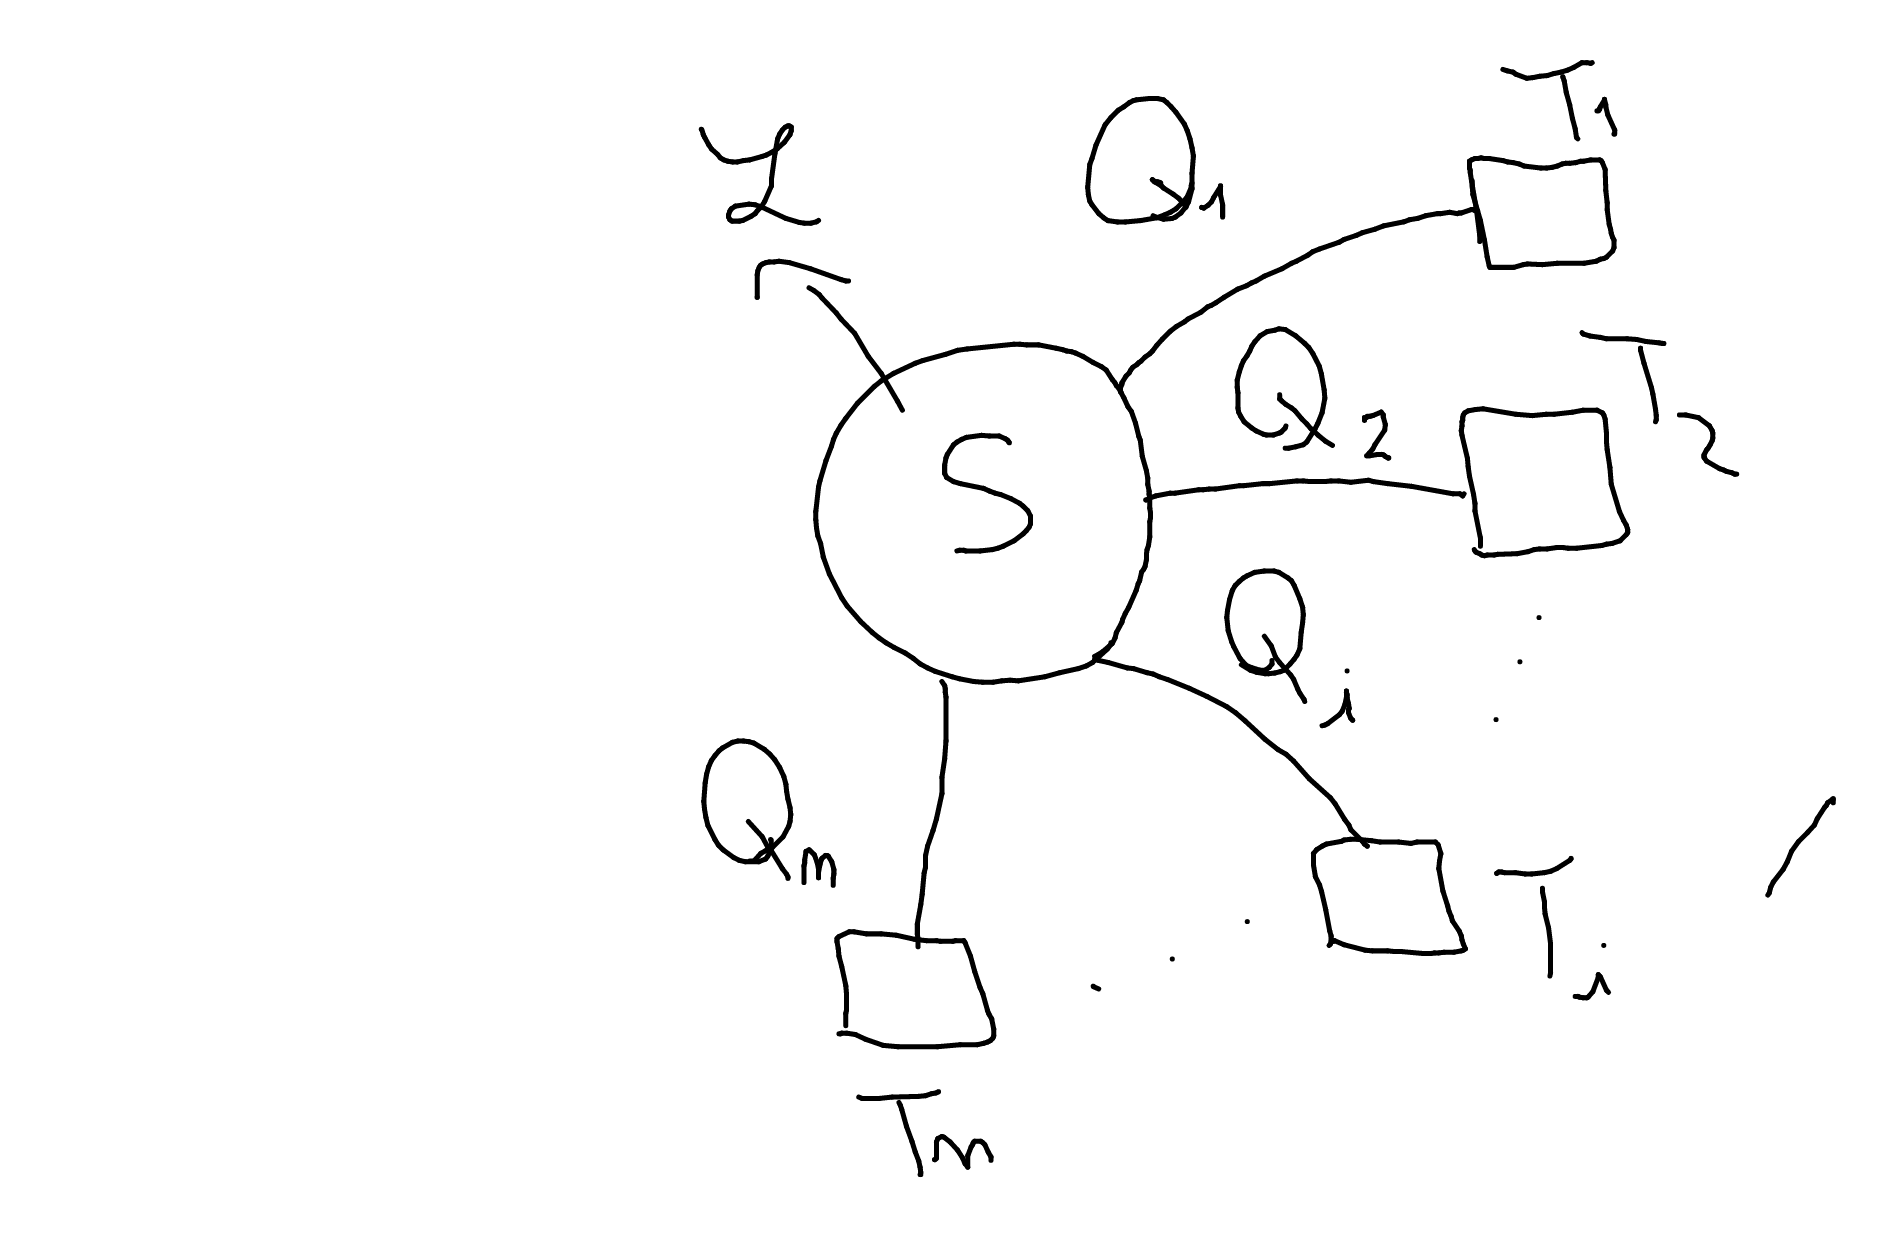
\includegraphics[width=0.5\textwidth]{TeoremaClausius1.png}
    \label{TeoremaClausius1}
\end{figure}
Introduciamo poi n macchine di Carnot reversibili che lavorano tra una sorgente a temperatura $T_0$ e l'i-esima sorgente a temperatura $T_i$, scambiando rispetivamente un certo calore $Q_{i0}$ con la prima sorgente e $-Q_i$ con le altre:
\begin{figure}[H]
    \centering
    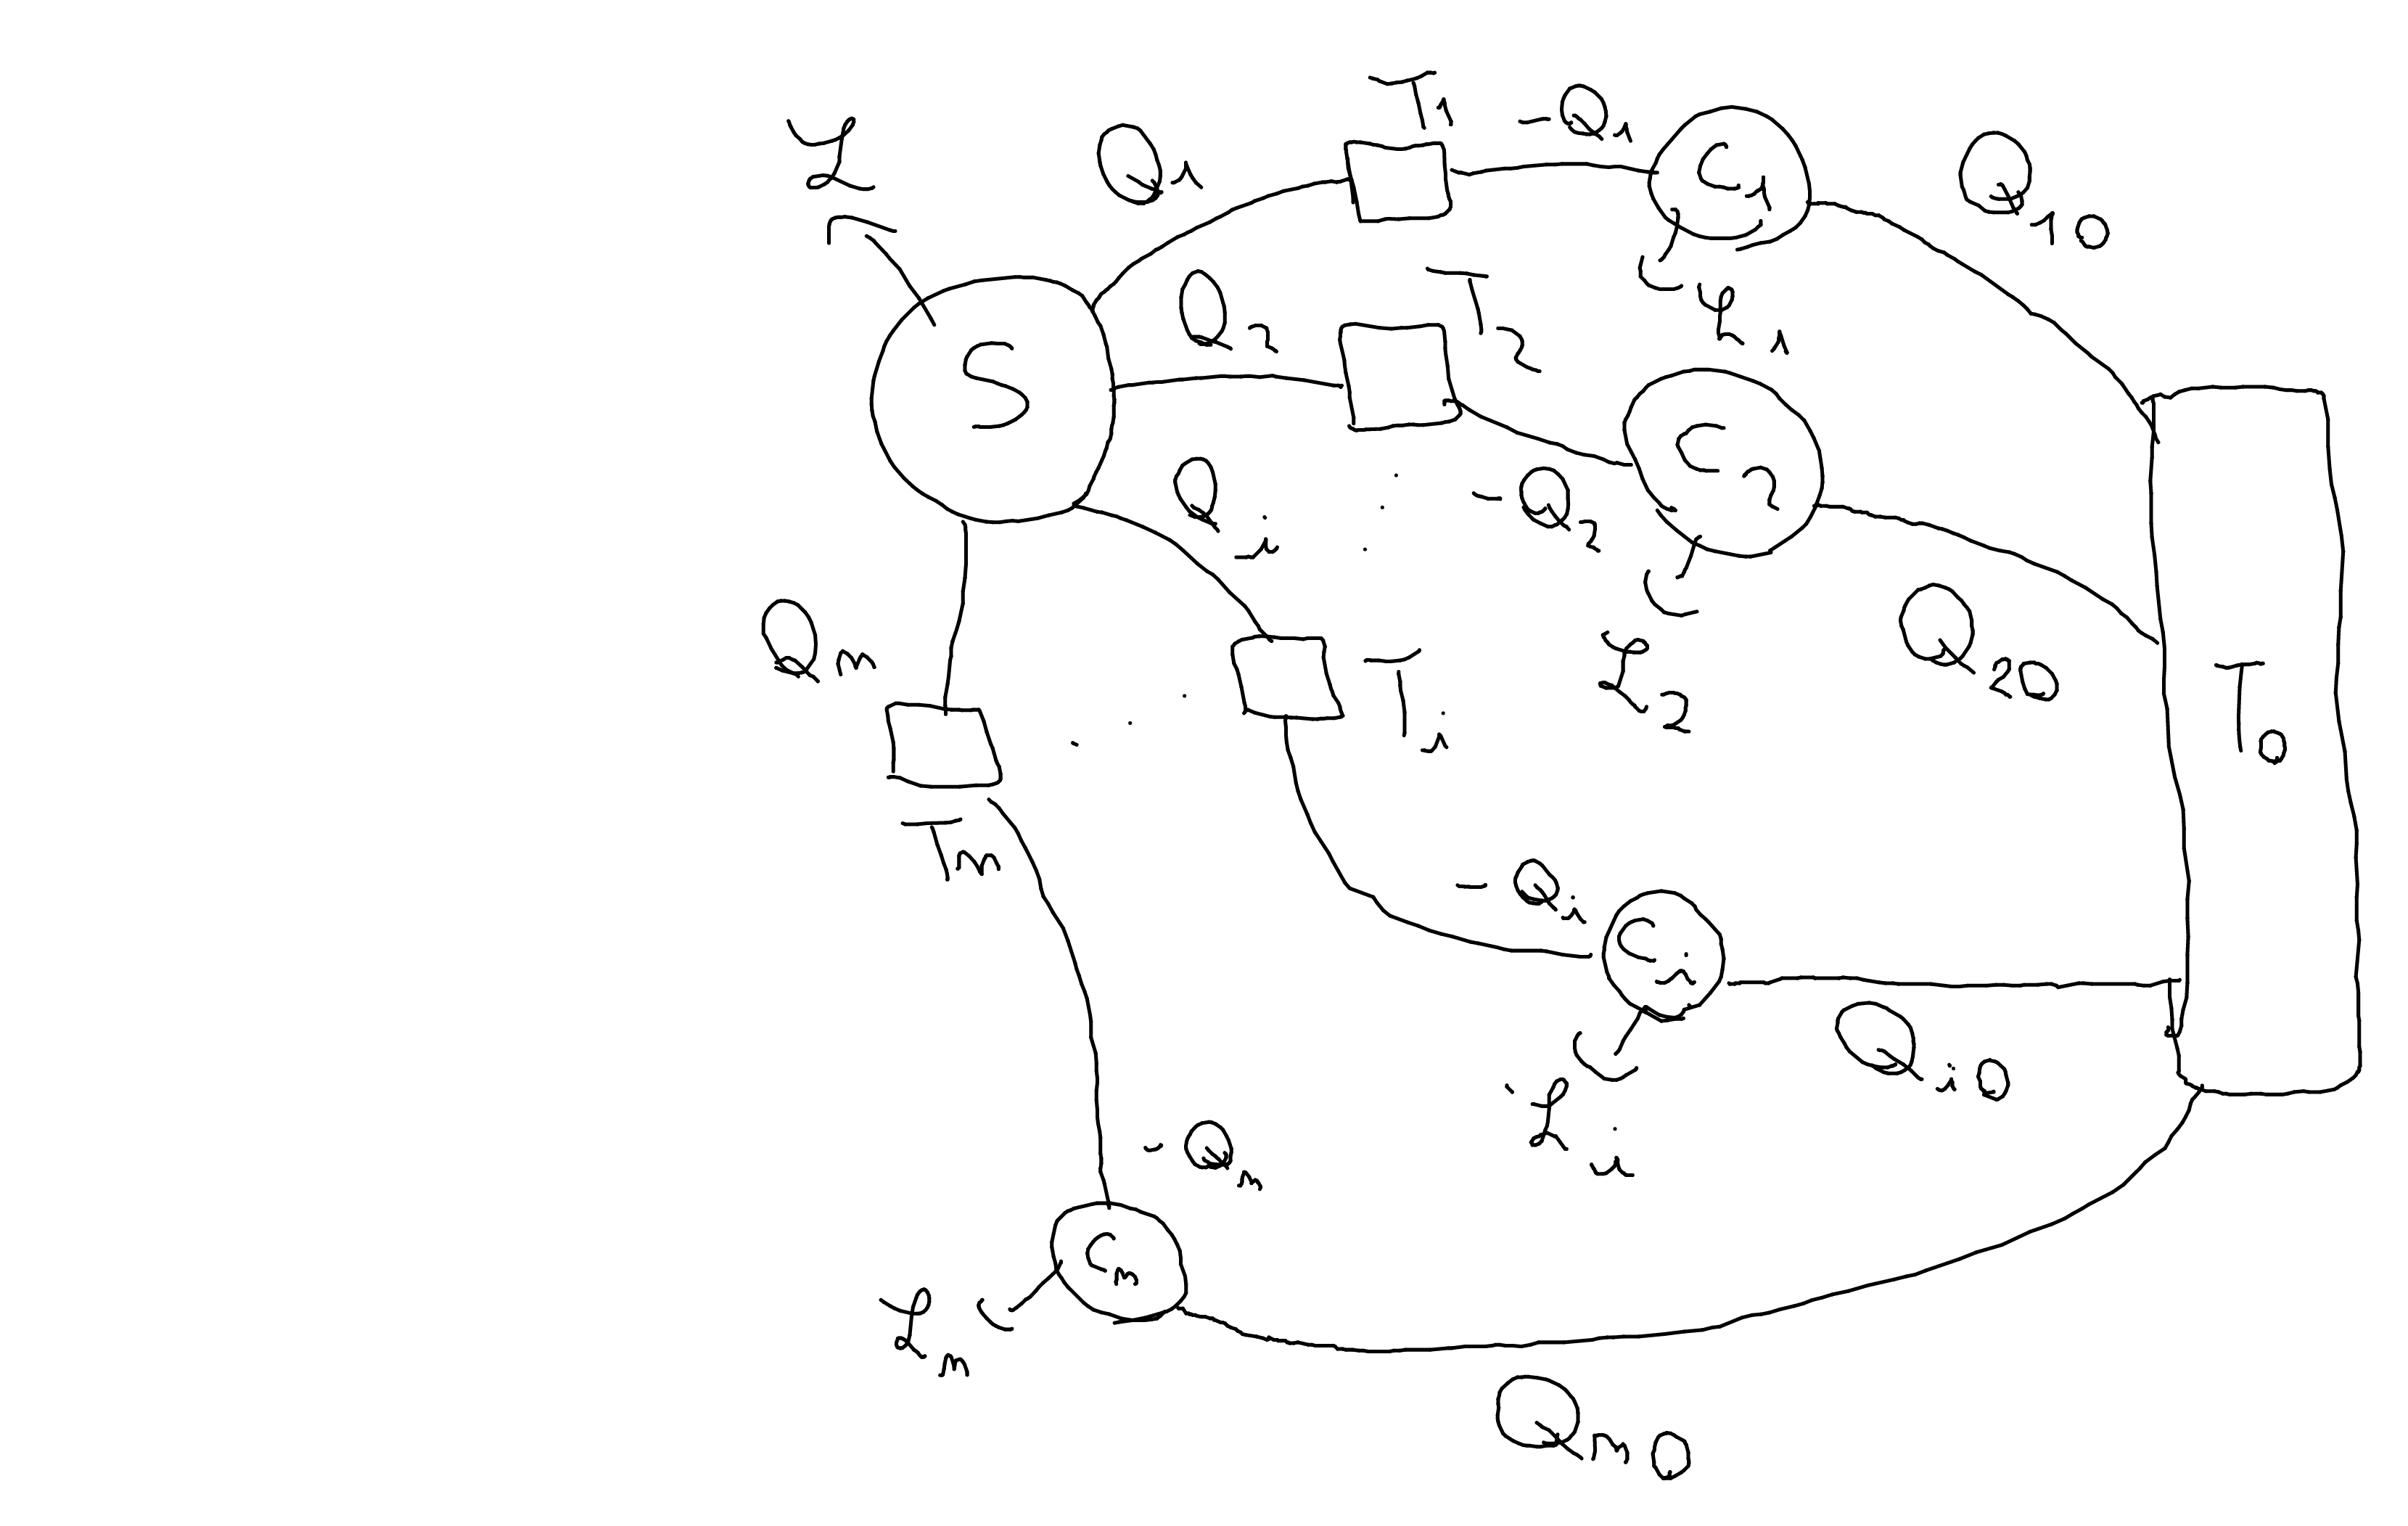
\includegraphics[width=0.5\textwidth]{TeoremaClausius2.png}
    \label{TeoremaClausius2}
\end{figure}
Abbiamo quindi effettivamente circuitato le sorgenti, ossia abbiamo costruito una nuova macchina termica che compie una trasformazione ciclica. Il calore totale scambiato dalla sorgente a temperatura $T_0$ deve essere tuttavia \textbf{ceduto} (o nullo) per l'enunciato di Kelvin (in quanto se fosse positivo l'unico risultato della trasformazione ciclica sarebbe il lavoro del sistema). Inoltre per il Teorema di Carnot applicato a ciascuna delle macchine termiche $C_i$ otteniamo:
\[-\frac{Q_i}{T_i}+\frac{Q_{i0}}{T_0}=0\then \frac{Q_{i0}}{T_0}=\frac{Q_i}{T_i}\]
Sommando sull'indice i otteniamo (detto $Q_0$ il calore totale ceduto dalla sorgente a temperatura $T_0$):
\[\sum_i\frac{Q_i}{T_i}=\sum_i\frac{Q_{i0}}{T_0}=\frac{Q_0}{T_0}\leq0\then \boxed{\frac{Q_i}{T_i}\leq0}\]
Questa relazione è nota come \textbf{disuguaglianza di Clausius}. Nel caso particolare in cui la macchina termia S compia una trasformazione ciclica reversibile otteniamo:
\begin{equation}
\boxed{\sum_i\frac{Q_i}{T_i}=0}
\end{equation}
Per un numero arbitrariamente grande di sorgenti (e quindi macchine di Carnot) otteniamo invece l'\textbf{integrale di Clausius} per una macchina reversibile:
\begin{equation}
    \boxed{\oint\frac{\delta Q}{T_{sorgente}}=\oint\frac{\delta Q}{T}=0}
\end{equation}
Che consiste nell'approssimare un qualunque ciclo con dei cicli di Carnot:
\begin{figure}[H]
    \centering
    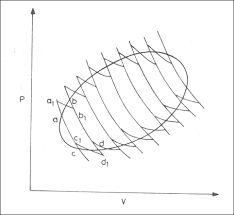
\includegraphics[width=0.3\textwidth]{IntegraleClausius.png}
    \caption{Approssimazione di un qualunque Ciclo Reversibile con dei Cicli di Carnot}
    \label{IntegraleClausius}
\end{figure}
In generale vale la disuguaglianza:
\begin{equation}
\boxed{\oint\frac{\delta Q}{T}\leq0}
\end{equation}
\end{thm}
\begin{prop}[Generalizzazione ad una Trasformazione Aperta]
Dal teorema di Clausius ricaviamo l'importante risultato che è l'integrale o la somma di Clausius, entrambe uguali a 0 per macchine reversibili:
\[\oint\frac{\delta Q}{T}=0\quad\sum_i\frac{Q_i}{T_i}=0\]
Dall'integrale di Clausius si può dimostrare che esiste una funzione di stato S tale che:
\begin{equation}
\boxed{\dif S=\frac{\delta Q}{T}}
\end{equation}
Questa funzione di stato prende il nome di \textbf{entropia}.
Consideriamo ora una generica trasformazione AB (schematizzata in figura come irreversibile) e immaginiamo di compiere una trasformazione reversibile BA in modo tale da ottenere un ciclo. 
\begin{figure}[H]
    \centering
    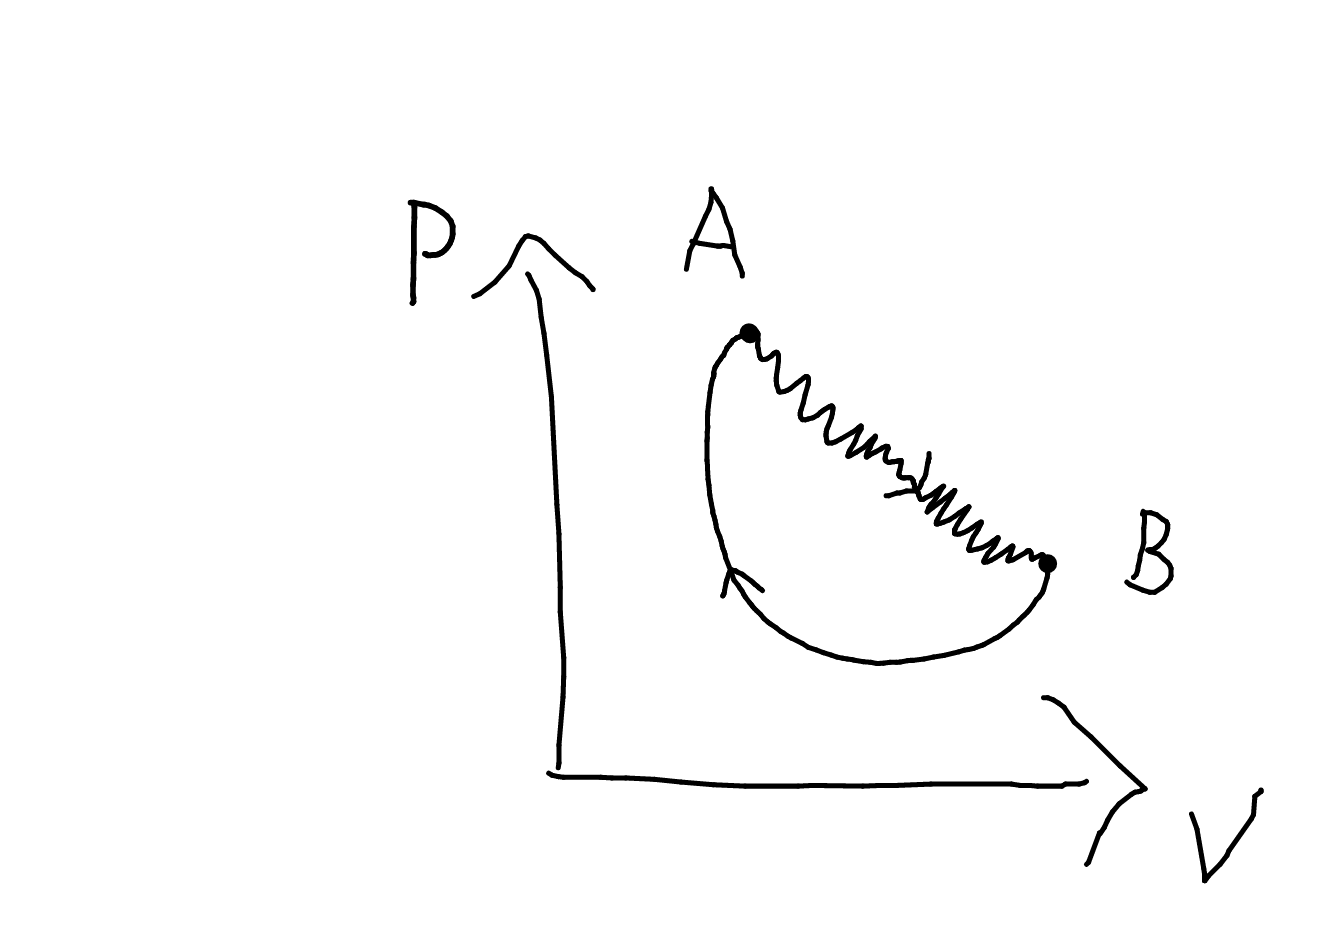
\includegraphics[width=0.5\textwidth]{TrasfAperta.png}
    \label{TrasformazioneAperta}
\end{figure}
Possiamo quindi applicare la disuguaglianza integrale nel caso generale esplicitando l'integrale:
\begin{equation}
\begin{split}
    \oint\frac{\delta Q}{T}&=\int_A^B\frac{\delta Q_{irr}}{T_S}+\int_B^A\frac{\delta Q_{rev}}{T}=\\
    &=\int_A^B\frac{\delta Q_{irr}}{T_S}+\int_B^A\dif S=\int_A^B\frac{\delta Q_{irr}}{T_S}-\int_A^B\dif S=\\
    &=\int_A^B\frac{\delta Q_{irr}}{T_S}-\left[S(B)-S(A)\right]\leq 0
\end{split}
\end{equation}
Otteniamo quindi:
\[\boxed{\int_A^B\frac{\delta Q_{irr}}{T_S}\leq S(B)-S(A)}\]
Che rappresenta la forma più generale della disuguaglianza di Clausius e rappresenta una formulazione matematica del secondo principio della termodinamica, includendo un importante risultato matematico (l'esistenza della funzione di stato \textbf{entropia}) e uno fisico (la disuguaglianza, ottenuta dall'enunciato di Kelvin).
\end{prop}
\note Nel caso di n sorgenti vale invece:
\[\sum_i\frac{Q_i}{T_i}\leq S(B)-S(A)\]
Inoltre, essendo l'entropia una funzione di stato, è possibile calcolarla direttamente solo per trasformazioni reversibili, mentre per quelle \textbf{irreversibili} si può calcolare \textit{combinando le variazioni di entropia di altre due trasformazioni reversibili}.
\subsubsection{La Variazione di Entropia di Alcune Trasformazioni}
\paragraph{Solidi e Liquidi}
Durante le trasformazioni di fase il calore scambiato con una certa massa di sostanza vale:
\[Q=\pm m\lambda\]
Calcoliamo l'integrale di Clausius:
\begin{equation}
    \Delta S=\int \frac{\dif Q_{rev}}{T_0}=\frac{Q}{T_0}=\pm\frac{m\lambda}{T_0}
\end{equation}
Quando invece i solidi e liquidi passano da una temperatura all'altra:
\[\Delta S=\int_A^B\frac{\delta Q}{T}=mc\int_A^B\frac{\dif T}{T}=mc\ln\frac{T_B}{T_A}\]
\paragraph{Trasformazioni Reversibili dei Gas}
Per ogni trasformazioni reversibile possiamo applicare il seguente ragionamento:
\begin{equation}
\begin{split}
    \dif S&=\frac{\delta Q_{rev}}{T}=n\overline{c}_V\frac{\dif T}{T}+\frac{1}{T}p\dif V=\\
    &=n\overline{c}_V\frac{\dif T}{T}+\frac{1}{T}\frac{nRT}{V}\dif V=\\
    &=n\overline{c}_V\frac{\dif T}{T}+\frac{nR}{V}\dif V=n\overline{c}_V\frac{\dif T}{T}+nR\frac{\dif V}{V}=\\
    &=n\overline{c}_V\left[\frac{\dif T}{T}+\frac{\overline{c}_p-\overline{c}_V}{\overline{c}_V}\frac{\dif V}{V}\right]=\\
    &=n\overline{c}_V\left[\frac{\dif T}{T}+(\gamma-1)\frac{\dif V}{V}\right]
\end{split}
\end{equation}
Calcoliamo ora l'integrale di Clausius:
\begin{equation}
\begin{split}
    \Delta S&=\int_A^B\dif S=\int_A^Bn\overline{c}_V\left[\frac{\dif T}{T}+(\gamma-1)\frac{\dif V}{V}\right]=\\
    &=n\overline{c}_V\int_A^B\left[\frac{\dif T}{T}+(\gamma-1)\frac{\dif V}{V}\right]=\\
    &=n\overline{c}_V\left[\ln\frac{T_B}{T_A}+(\gamma-1)\ln\frac{V_B}{B_A}\right]=\\
    &=n\overline{c}_V\left[\ln\frac{T_B}{T_A}+\left(\ln\frac{V_B}{B_A}\right)^{\gamma-1}\right]=\\
    &=n\overline{c}_V\ln\left[\frac{T_B}{T_A}\left(\frac{V_B}{B_A}\right)^{\gamma-1}\right]=\\
    &=n\overline{c}_V\ln\left[\frac{T_BV_B^{\gamma-1}}{T_AV_A^{\gamma-1}}\right]
\end{split}
\end{equation}
Possiamo quindi esprimere in tre modi la variazione di entropia:
\[\Delta S=n\overline{c}_V\ln\left[\frac{T_BV_B^{\gamma-1}}{T_AV_A^{\gamma-1}}\right]=n\overline{c}_V\ln\left[\frac{p_BV_B^{\gamma}}{p_AV_A^{\gamma}}\right]=n\overline{c}_V\ln\left[\frac{T_A^{\gamma}T_B^{\gamma}}{p_A^{\gamma-1}p_B^{\gamma-1}}\right]\]
Esaminiamo ora singolarmente le maggiori trasformazioni reversibili.\\
L'\textbf{adiabatica} è la più semplice, in quanto è caratterizzata da $pV^{\gamma}=cost$, quindi otteniamo:
\[\Delta S=n\overline{c}_V\ln\left[\frac{p_BV_B^{\gamma}}{p_AV_A^{\gamma}}\right]=n\overline{c}_V\ln(1)=0\]
Ossia una trasformazione adiabatica è \textbf{isoentropica}, non cambia mai il proprio valore di Entropia.
Per quanto riguarda l'\textbf{isocora}:
\[\Delta S=n\overline{c}_V\ln\left[\frac{T_BV_B^{\gamma-1}}{T_AV_A^{\gamma-1}}\right]=n\overline{c}_V\ln\frac{T_B}{T_A}=n\overline{c}_V\ln\frac{p_B}{p_A}\]
L'\textbf{isobara}:
\[\Delta S=n\overline{c}_V\ln\left[\frac{p_BV_B^{\gamma}}{p_AV_A^{\gamma}}\right]=n\overline{c}_V\gamma\ln\frac{V_B}{V_A}=n\overline{c}_V(\frac{\overline{c}_p}{\overline{c}_V})\ln\frac{V_B}{V_A}=n\overline{c}_p\ln\frac{V_B}{V_A}=n\overline{c}_p\ln\frac{T_B}{T_A}\]
E infine l'\textbf{isoterma}:
\[\Delta S=n\overline{c}_V\ln\left[\frac{T_BV_B^{\gamma-1}}{T_AV_A^{\gamma-1}}\right]=n\overline{c}_V(\gamma-1)\ln\frac{V_B}{V_A}=n\overline{c}_V(
\frac{\overline{c}_p-\overline{c}_V}{\overline{c}_V})\ln\frac{V_B}{V_A}=n(\overline{c}_p-\overline{c}_V)\ln\frac{V_B}{V_A}=nR\ln\frac{V_B}{V_A}=nR\ln\frac{p_A}{p_B}\]
\paragraph{Espansione Libera}
Studiamo ora il caso dell'Espansione Libera di un gas come nel Secondo Esperimento di Joule. Siccome l'entropia è una funzione di stato possiamo applicare il risultato ottenuto anche ad una trasformazione irreversibile (come è tal caso) e otteniamo:
\begin{equation}
\Delta S=n\overline{c}_V\ln\left[\frac{T_fV_f^{\gamma-1}}{T_iV_i^{\gamma-1}}\right]=n\overline{c}_V\ln\frac{V_f^{\gamma-1}}{V_i^{\gamma-1}}=nR\ln\frac{V_f}{V_i}=nR\ln\frac{V_B+V_A}{V_A}>0
\end{equation}
Notiamo che la variazione di entropia è positiva, come ci si aspettava. 
\paragraph{Equilibrio Termico di due Corpi}
Dati due corpi a temperatura $T_A$ e $T_B$ rispettivamente, il calore che si scambiano è:
\[\delta Q_A=m_Ac_A\dif T\quad\delta Q_B=m_Bc_B\dif T\]
Calcoliamo l'integrale di Clausius tra lo stato iniziale e quello di equilibrio:
\[\Delta S=\Delta S_A+\Delta S_B=m_Ac_A\ln\frac{T_e}{T_A}+m_Bc_B\ln\frac{T_e}{T_B}\]
Si può dimostrare che in generale questa quantità è positiva utilizzando le proprietà dei logaritmi, considerando il caso in cui i corpi abbiano uguale massa e stesso calore specifico:
\begin{equation}
\begin{split}
    \Delta S&=mc\ln\left[\frac{(T_A+T_B)^2}{T_AT_B}\right]=\\
    &=2mc\ln\left[\frac{T_A+T_B}{\sqrt{T_AT_B}}\right]>0
\end{split}
\end{equation}
L'argomento è maggiore di 1 in quanto si può dimostrare che la media aritmetica è maggiore della media geometrica degli stessi valori. 

\paragraph{Tabella delle Trasformazioni Reversibili}
\begin{center}
\scalebox{1.5}{
\begin{tabular}{|c|c|c|c|c|}
    \hline
    \textbf{Trasformazione} & \textbf{Q} & \textbf{L} & \textbf{$\Delta U$} & \textbf{$\Delta S$}  \\
    \hline
    Isobara & $n\overline{c}_p\Delta T$ & $p_A(V_B-V_A)$ & $n\c_V\Delta T$ & $n\c_p\ln\frac{T_B}{T_A}$ \\
    \hline
    Isocora & $n\c_V\Delta T$ & 0 & $n\c_V\Delta$ & $n\c_v\ln\frac{T_B}{T_A}$\\
    \hline
    Isoterma & $L$ & $nRT\ln\frac{V_B}{V_A}$ & 0 & $nR\ln\frac{V_B}{V_A}$\\
    \hline
    Abiabatica & 0 & $-n\c_V\Delta T$ & $n\c_V\Delta T$ & 0\\
    \hline
\end{tabular}}
\end{center}







\end{document}